% Master Thesis Automation and Control DTU Template
% Remus M. Prunescu rmpr@elektro.dtu.dk
% 2013

\documentclass[a4paper,11pt]{memoir}

% Include all settings
% Add packages
\usepackage[T1]{fontenc}
\usepackage[utf8]{inputenc}
\usepackage[czech, danish, english]{babel}
\usepackage{graphicx}
\usepackage{microtype}
\usepackage{lmodern}
\usepackage{lipsum}
\usepackage[intoc]{nomencl} % Nomenclature package
\usepackage{color}
\usepackage{times}
\usepackage{textcomp}
\usepackage{hyperref}
\usepackage{textpos}
\usepackage{indentfirst}
\usepackage{tikz}
\usepackage{pgfplots}
\usepackage{ifthen}
\usepackage{float}
%\usepackage{mathtools}\textbf{}
% subfigures
\usepackage{booktabs}
\usepackage{caption}
\usepackage{subcaption}
\usepackage{epstopdf}

\usepackage{graphicx}
\usepackage{epstopdf}
\usepackage{amsmath}
\usepackage{varioref}
\usepackage{todonotes}
\usepackage{colortbl}
\usepackage{nomencl}
\usepackage{algorithm}
\usepackage{algpseudocode}
\floatname{algorithm}{Procedure}
\usepackage{dirtree}

% Enable subfigures
\newsubfloat{figure}

% Path to graphics
\graphicspath{{figures/}}

\everymath{\displaystyle}

% Avoid a warning
\pdfminorversion=5

% Define layout dimensions

\setlrmarginsandblock{35mm}{25mm}{*}
\setulmarginsandblock{30mm}{30mm}{*}
\setheadfoot{8mm}{10mm}
\checkandfixthelayout
\OnehalfSpacing

\usepackage[backend=biber,style=numeric]{biblatex}


% Create a theorem environment
\newtheorem{theorem}{Theorem}

% Chapter style
\chapterstyle{madsen}

% Section numbering depth
\maxtocdepth{subsection}
\maxsecnumdepth{subsection}

% Enable nomenclature
\makenomenclature


% Enable line numbering
%\usepackage{lineno}
%\pagewiselinenumbers
%\modulolinenumbers[5]


% Change table of contents name
\addto\captionsenglish{% Replace "english" with the language you use
	\renewcommand{\contentsname}%
	{Table of Contents}%
}

% Make floats name bold
\captionnamefont{\bfseries}

% Get a signature command
\makeatletter
\newcommand*{\getlength}[1]{\strip@pt#1}
\makeatother

\newlength{\signlength}
\setlength{\signlength}{0.5\textwidth}

\newcommand{\signature}[1]{%
\noindent \line(1,0){\getlength{\signlength}}\\
\noindent #1
}

% Add measuring units to nomenclature
\newcommand{\nomunit}[1]{\renewcommand{\nomentryend}{\hspace*{\fill}#1}}

\captionstyle{\OnehalfSpacing}


% Company logo
\def\bCompanyLogo{true}

% A fix for memoir-kluwer
\renewcommand{\bf}{\textbf}

\newcommand{\titledate}[2][2.5in]{%
    \vspace{2 cm}
    \noindent%
    \begin{tabular}{@{}p{#1}@{}}
        \\ \hline \\[-.75\normalbaselineskip]
        #2
    \end{tabular} \hspace{0.5in}
    \begin{tabular}{@{}p{#1}@{}}
        \\ \hline \\[-.75\normalbaselineskip]
        Date
    \end{tabular}
}
\bibliography{references}
% Define thesis data
\def\ThYear{2016}

\def\ThTitleEN{Mapping of dynamic environments for effective navigation of mobile robots}
%\def\ThSubtitleEN{}
%\def\ThTitleDK{Min dejlige projekt}
%\def\ThSubtitleDK{Min super undertitel}

\def\ThAuthors{Anders Birkehøj Jensen\\ Martin Groth Albøge}

\def\ThSupervisors{Lars-Peter Ellekilde, 
	Lektor at the Mærsk Mc-Kinney Møller Instituttet of SDU\\ Niels Jul Jacobsen, CTO at Mobile Industrial Robots ApS}
\def\ThDepartment{\textbf{SDU Robot Systems}\\ Mærsk Mc-Kinney Møller Instituttet\\ University of Southern Denmark\\ Campusvej 55\\ 5230 Odense M\\ Denmark\\ Tel: +45 6550 3541}

%\def\ThElektroEmail{studievejledning@tek.sdu.dk}
\def\ThBeginDate{Septemper 2015}
\def\ThEndDate{June 2016}
\def\ThProjectPeriod{\ThBeginDate - \ThEndDate}
\def\ThECTS{40}
\def\ThEducation{MSc}
\def\ThField{Robot Systems}
%\def\ThClass{Confidential until October 1st, 2016}
\def\ThRemarks{This report is submitted as partial fulfillment of the requirements for graduation in the above education at the University Southern of Denmark.}
%\def\ThCopyrights{\copyright Remus M. Prunescu, \ThYear}

\begin{document}

\begin{titlingpage}
	\thispagestyle{empty}
	\enlargethispage{1.3cm}
	\calccentering{\unitlength}
	\begin{adjustwidth}{\unitlength}{-\unitlength}
		\vspace*{-1.9cm}
		\begin{figure} %
			\centering
			\includegraphics[width=0.5\textwidth]{figures/front_matter/SDU2013_SDU_Logo}
		\end{figure}

		\begin{centering}
			\vspace{\stretch{2}}
			%{\Huge\sffamily\ThAuthors\\[2cm]}
			\begin{Spacing}{1.2}
				{\sffamily\HUGE\textbf{\ThTitleEN}\\[1cm]}
				{\sffamily\LARGE{MSc. Robot Systems}\\[1cm]}
				{\sffamily\LARGE{Master's Thesis, \ThEndDate}\\[1cm]}
			\end{Spacing}
			%\vspace{\stretch{1}}
			{\LARGE\sffamily\ThAuthors\\[2cm]}
			\vspace{\stretch{2}}
		\end{centering}
		\begin{raggedright}
			\sffamily\LARGE{Mærsk Mc-Kinney Møller Instituttet}
			\ifthenelse{\equal{\bCompanyLogo}{true}}{%
				\begin{textblock}{3}(9,-0.85) %
					\includegraphics[width=\textwidth]{figures/front_matter/mir_logo}
				\end{textblock}
			}{} % End if
		\end{raggedright}
	\end{adjustwidth}

	\cleardoublepage

	\thispagestyle{empty}
	\enlargethispage{1.3cm}
	\calccentering{\unitlength}
	\begin{adjustwidth}{\unitlength-0.4cm}{-\unitlength-0.4cm}
		\begin{center}
			\vspace{\stretch{1}}
			\vspace{1.5cm}
			{\Huge\scshape\ThAuthors}\\[2cm]
			\begin{Spacing}{3}
				{\sffamily\HUGE\textbf{\ThTitleEN}}\\[1cm]
%				{\sffamily\LARGE\textbf{{\ThSubtitleEN}}}\\[1cm]
				{\sffamily\LARGE{Master's Thesis, \ThEndDate}}\\[2cm]
			\end{Spacing}
			\vspace{\stretch{2}}
			\begin{Spacing}{1.5}
				{\Large Supervisors:}\\
				{\Large\ThSupervisors\\}
			\end{Spacing}
			\vspace{\stretch{3}}
			{\sffamily SDU - University of Southern Denmark, Odense - \ThYear}\\[1cm]
			\vspace{\stretch{4}}
		\end{center}
	\end{adjustwidth}

	\cleardoublepage
	\thispagestyle{empty}
	\calccentering{\unitlength}
	\begin{adjustwidth*}{\unitlength}{-\unitlength}
		\textbf{\ThTitleEN}
		\vspace{\stretch{1}}

		\noindent\textbf{This report was prepared by:}\\
		\ThAuthors

		\vspace{\stretch{2}}

		\noindent\textbf{Advisors:}\\
		\ThSupervisors

		\vspace{\stretch{3}}

		\noindent\ThDepartment

		\vspace{\stretch{4}}

%		\noindent\ThElektroEmail

		\vspace{\stretch{5}}

		\noindent{\renewcommand{\arraystretch}{2}\begin{tabular}{@{}lp{0.75\textwidth}}
			Project period:&	\ThProjectPeriod\\
			ECTS:&		\ThECTS\\
			Education:&	\ThEducation\\
			Field:&		\ThField\\
%			Class:&		\ThClass\\
			Remarks:&	\ThRemarks\\
%			Copyrights:&\ThCopyrights
		\end{tabular}}
	\end{adjustwidth*}
\end{titlingpage}

\frontmatter

\tableofcontents*

\cleardoublepage
\listoffigures
\cleardoublepage
\listoftables
\listoftodos

%!TEX root = ../../report.tex
\chapter*{Abstract}
\printnomenclature

\mainmatter
%!TEX root = ../../report.tex
\chapter{Introduction}

Mobile robot navigation today is highly based on offline generated maps of the environment. This is adequate in a lot of applications, but this approach has issues. As the discrepancy between the internal map of the robot and the true state of the environment increases, tasks like path planning and localization will be based on more and more erroneous data. To overcome these challenges it would be beneficial to incorporate the dynamics into the perception the robot has of the world.

As the environment changes a robot which navigation is based on a predetermined static map will be prone to plan paths where there might be placed an obstacle since the map was generated and the time of planning. This will force the robot to replan the path thus wasting time or causing the robot to fail to reach its goal. Likewise will a map based navigation be subject to errors as the map increasingly misrepresents the environment. The most simple solution to these problems would be to add or remove obstacles based on the last observation. This, however, will likely clutter the map with highly dynamical obstacles like people moving through or vehicles driving by and thus has a high risk of blocking large parts of the map. Therefore it is necessary to consider which obstacle should be included and which should be left out and furthermore how this selection is to be done. The question of how relates to another consideration, namely how are obstacles and the environment represented in the robot.

\section{Simultations Location and Mapping}
The SLAM problem \\
Static \\ 
Dynamic \\

\subsection{Long-term SLAM}

New stuff\\
Long term navigation dynamic environment
- Wrong / suboptimal path planning
- Failed localization

Requirements
Plasticity
- Adapt quickly to changes 
- Avoid insertion errors -> recursion problem (localization on updated map -> new map based on localization)
- Avoid bad landmarks

Pre- assumption
2D world
Lidar sensor only
Preferably an easy interface 
Changes in the environment are continuos and partial. Areas are visited more frequently than significant changes. (change per visit?)

It should be able to run online
Nice: low resource requirements





%!TEX root = ../../report.tex
\chapter{Problem Analysis}
% \cite{tdoa_book}
This chapter investigates MIR’s exiting software related to global maps of environments. The investigation is conducted by interviewing the CTO at MIR, Niels Jul Jacobsen and through experiments with the source code for MIR100. It reveals some inefficiencies in the current implementation where a static map is used for localization and navigation in a dynamic environment.
% introduce the dynamic map and keep consitent with it

% \cite{tdoa_book}
\section{Path Planning in Dynamic Environments}
–	Generelt problem – planning I dynamiske miljøer


\subsection{Costmap in path planner}
Plans a path through a grid based map with the lowest possible cost. 
cost -> obstacles, obstacle vicenity, user-definements

MIR enables users to refine the static map by inserting costs that control the paths the robot follows. It is as an example possible to insert non-lethal or lethal obstacles in it. These user-preferences should also be present in a dynamic map.

\subsection{Ineffective Global Navigation in Static Maps}
Previously use static map in dynamic environments -> replan


Too much MIR
When the MIR100 navigates, it plans a global obstacle free path in the static map. In case the path goes through obstacles, since they are not present in the static map, the local planner will try to avoid the obstacle, while trying to follow the global path as good as possible. In some cases, the local planner might be stuck in a blocked corridor and hence recovery behaviors must try to find a solution. This is both ineffective and annoying for users (Kilde Niels). This can be avoided by adding observed obstacles to the static map, but by doing so the map might be cluttered with highly dynamic obstacles, which makes it impossible to plan a path. Therefore, the highly dynamic obstacles should not be included in the map. 




%!TEX root = ../../report.tex
\section{Characteristics in industrial environments}

\subsection{Highly Dynamically Moving Objects}
60 seconds
Humans, animals, vehicles
Objects moving within the field of view of the robot.
\subsection{Semi-Static Obstacles}
Objects that moves without field of view of the object.
Parked vehicles, pallets, standing humans, doors, 
\subsection{Static Obstacles}
Steady for weeks
fixedly mounted equipment like a New wall, heavy machinery
Significant probability for observing a obstacle in the next observation.


%!TEX root = ../../report.tex
\section{Timing and measurements}

\subsection{Dependency of Measurements}
If Time scales on Laser scan measurements is much less than the time between movements, then it is very likely that consecutive measurements are the same. So when trying to observe whether obstacles have moved or not, each measurement is not very describing.
\subsection{Partial Observability}
When trying to model the dynamics of the environment it would be ideal to be able to observe the entire environment all the time to make sure all changes would be observed. This is of cause impossible in all but the most simple test setups and consequently this problem of partial observability must be considered and solved or at least, the effects of it should be minimized.

It is impossible to estimate the dynamic of an obstacle if it moves in between observations.


%%!TEX root = ../../report.tex
\section{Uncertainties in Mapping}

\subsection{LiDar sensors}
Sensor model Different reasons to errors:

Too long measurements when no reflexion.

Very small angle error(Kilde, evt. datablad)

Larger distance error Gaussian


\subsection{Localization}
Driftless localization

AMCL gives a covariance matrix. 

Jumps in localization
 % written in mapping with location noise

%!TEX root = ../../report.tex
\section{MIR 100 platform}

Drives almost constantly with 5 km/h.

\subsection{LiDar}
LiDar in 16 cm height

Range = 30m

LiDar type: SICK S30B-2011ca

std. deviation = 1cm.

\subsection{AMCL localization}
MIR uses a ROS implementation of the adaptive monte carlo localization (AMCL), which uses a particle filter to track the pose of a robot against a known map (http://wiki.ros.org/amcl ). Today this is done by matching laser range scans with a static map. In dynamic environments with mismatch between the observed world and the map, the localization would be wrong. By adding semi static obstacles to the map the amount of mismatches is lowered, but location would still be wrong in highly unpredictable regions. It would be advantageous to identify these regions to take proper precautions.






%!TEX root = ../../report.tex
\chapter{Mapping of Static environments}
This chapter investigates improved mapping of static environments with LIDAR sensors by incorporating sensor and localization noise. 
Specifically the following aim is considered:

\begin{enumerate}
    \setcounter{enumi}{0}
    \item Precise mapping of static environments by incorporating sensor and localization noise
\end{enumerate}

Mapping of static environments is an essential part of mobile robotics. It forms the basics for allowing the robot to navigate the environment. 
By integrating measurements with Bayes methods for a short period of time, where the local environment is likely to be static, the effects of sensor and localization errors can be reduced.
Figure \ref{fig:static_map_overview} shows the static mapping module in relation to the rest of the dynamic mapping system.  

\begin{figure}[htbp]
		\centering
		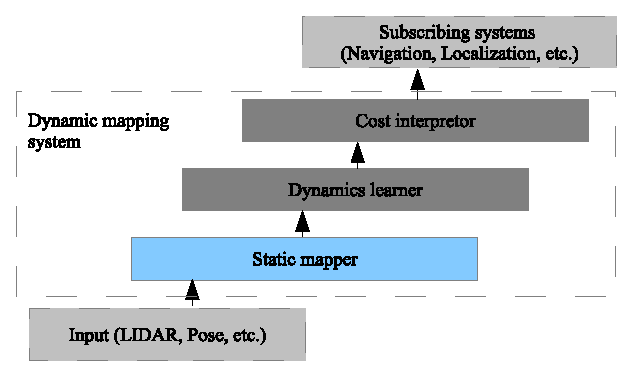
\includegraphics[scale=1]{chapters/static_mapping/figures/static_map_overview.eps}
		\caption{The static mapping in the dynamic mapping system}
		\label{fig:static_map_overview}
\end{figure}


%!TEX root = ../../report.tex
\section{Occupancy grid mapping}

An initial decision in mapping is how to represent the environment. A widely used method is the occupancy grid map, described in \cite{elfesMoravecOccGrid}. It splits the environment into evenly sized cells. Each cell contains an occupancy value describing probability the cell being occupied. 0 for completely free and 1 for completely occupied. An assumption in the occupancy grid map is that each cell is independent which is not strictly true but helps reduce the complexity of the mapping [**REFERENCE INSERT HERE***]. This can be expensive in memory as the entire environment is represented in the grid map. The benefit of the grid map is an ease of maintenance and good metric information \cite{mapbuildingSummary}. 
Another widely used representation is the topological map \cite{topologyOrig}. 
Herein the environment is represented as position or landmark nodes connected by vertices in a graph structure. 
This representation was created for effective navigation in the environment. 
A drawback of the topological map is that it contains less metric information than the occupancy grid mapping \cite{mapbuildingSummary}.

For the static mapping in this project there are other factors influencing the choice of representation. In the ROS system the grid map is already used and therefore the interfacing becomes significantly simpler and thus rendering the proposed mapping more easily integrated in other systems. The availability of metric information and the widespread use and therefore ease of integration makes the occupancy grid a favored choice in this project. 

hen mapping with an occupancy grid each observation is treated as independent and thus adds a contribution to the occupancy of the cell. The most simple mapping in occupancy grid will mark a cell in accordance to its last observation with the full value. If the cell is observed as occupied the cell value is set to 1 and 0 if it is observed free. Using this very simple mapping the last observation is fully in control of the cell value. This makes the method very susceptible to any form of noise. To avoid this, values based on a sensor model are often used to compensates for the noise in the sensor. 

In the occupancy grid a log-odds representation of the probability is used \cite{probRob}. In equation \ref{eq:log-odds} the calculation from probability to log-odds is shown. The value \(p(m_{occ}|z)\) is determined by the sensor model. 

\begin{equation}
\label{eq:log-odds}
l_{occ} =  log(\frac{p(m_{occ}|z)}{1-p(m_{occ}|z)} )
\end{equation}

where \(z\) is the observation and \(m_{occ}\) is the occupied state. 
\\
Using the log-odds representation the occupancy value of a cell is calculated by equation \ref{eq:occGrid_occCalc}. 

\begin{equation}
\label{eq:occGrid_occCalc}
cell_{occ} = \sum_{i} log(\frac{p(m_{occ}|z_i)}{1-p(m_{occ}|z_i)} )
\end{equation}



Why occupancy grid ? (interface, recognised, used through put the community - considerations on other representation)
Mapping by inserting obstacle and free when observed.
Independence - cells, measurements
Log odds
Real world test -> Results in bad maps.
Propagation of noise to avoid over confidence while still converging to the right solution. (Types of noise)


%!TEX root = ../../report.tex
\section{Laser range sensor}

Basics of sensor
Forward Sensor Model
What noise does the sensor introduce. (see prob robotics)
Ideal Inverse Sensor Model

Elfes Sensor Model
Reference to Elfes
Calculated through kernel density estimation. 
Considerations on the std deviation

%!TEX root = ../../report.tex
\section{Mapping with Location noise}

\subsection{Monte Carlo localization}

AMCL

Scan map with location noise and AMCL
Considerations on noise. What types of noise are present. Estimation of the noise. Comparison between estimation and actual error (of bags) 
Non-ideal Inverse Sensor Model
From hector

\subsection{Monte Carlo Integration Inverse Sensor Model}

\cite{monteCarloIntegration}

Cone Sensor Model
Based on sonar model. Used to incorporate pose noise. 
Simulation of Mapping with Location Noise
Comparison
Efficiency - Computational price
Map Score (obstacle centered and whole map, adjusted for number of cells)
\begin{figure}
	\centering
	\includegraphics[width=0.7\linewidth]{figures/static_mapping/particle_sensor}
	\caption{Example map with few scans from the five highest weighted particles.}
	\label{fig:particle_sensor}
\end{figure}

\begin{figure}
	\centering
	\begin{subfigure}[b]{0.45\textwidth}
		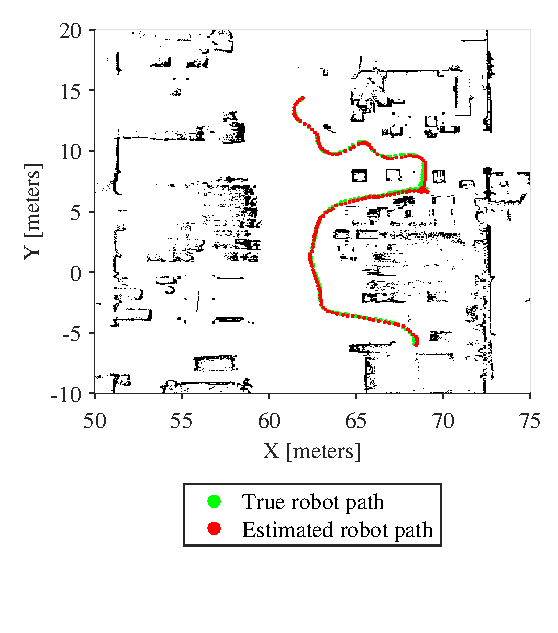
\includegraphics[width=\textwidth]{figures/static_mapping/map_with_poses}
		\caption{World represenation}
		\label{fig:simulated_robot_estimate_total}
	\end{subfigure}
	~ %add desired spacing between images, e. g. ~, \quad, \qquad, \hfill etc. 
	%(or a blank line to force the subfigure onto a new line)
	\begin{subfigure}[b]{0.45\textwidth}
		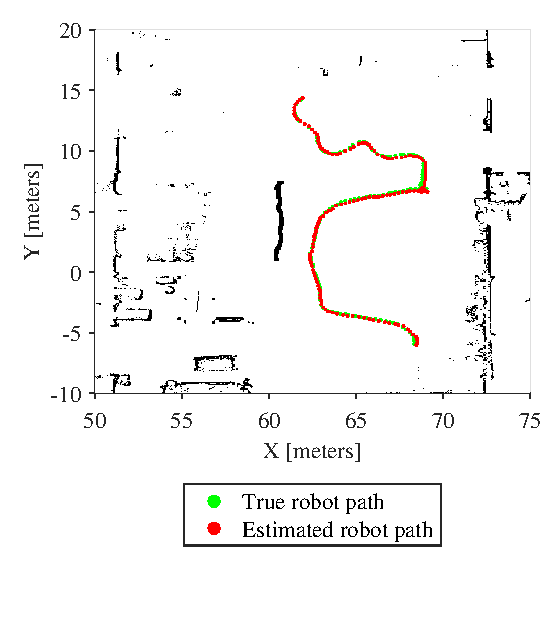
\includegraphics[width=\textwidth]{figures/static_mapping/amcl_map_with_poses}
		\caption{Map used by AMCL}
		\label{fig:simulated_robot_estimate_total_edited}
	\end{subfigure}
	\caption{Simulation of a MIR robot moving with imprecise location.}
	\label{fig:animals}
\end{figure}


%!TEX root = ../../report.tex
\section{Mapping an Industrial Environment}

Test setup 
Something about the scan environment
Mapping of the scan environment

Results

Conclusion

Observation: Jumps in localisation - must be considered and possibly suppressed

%!TEX root = ../../report.tex
\section{Summary}
In this chapter various different methods of including pose estimation noise into the mapping has been evaluated. The method that was ultimately chosen was in ideal sensor model but with reduced certainty for each observation. The occupancy values chosen for free is \(0.4\) and \(0.6\) for occupied. The pose estimation noise in incorporated as a weight that reduces the certainty as the estimation variance increases. The weight calculation can be seen in equation \ref{eq:pose-weight}. 
These elements has been inserted in the static mapper block, as seen in figure \ref{fig:static_map_detail}. 
The sensor input and pose estimation is combined and inserted in the static map as determined by the sensor model and noise weight. At fixed intervals the static map is then provided as a snapshot as output and cleared. 

\begin{figure}[htbp]
	\centering
	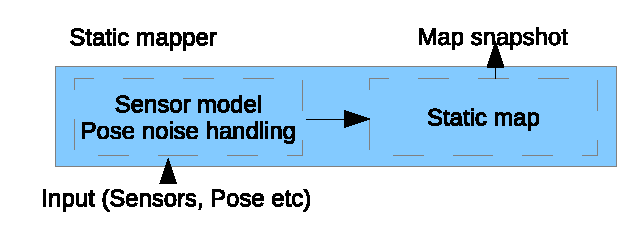
\includegraphics[scale=1]{chapters/static_mapping/figures/static_map_detail.eps}
	\caption{Static mapping module concept}
	\label{fig:static_map_detail}
\end{figure}


%!TEX root = ../../report.tex
\chapter{Mapping of Dynamic Areas}
\label{mapping_of_dynamic_areas}
This chapter investigates possible methods for learning the dynamic properties of an area in order to improve localization and navigation. The dynamic learner module is shown in figure \ref{fig:dynamic_learner_overview} in relation to the rest of the dynamic mapping system. The dynamic learner receives the static map snapshots and uses these as the basis for learning the dynamics.  


\begin{figure}[htbp]
	\centering
	\includegraphics[scale=1]{chapters/mapping_of_dynamic_areas/figures/dynamic_overview.eps}
	\caption{The static mapping in the dynamic mapping system}
	\label{fig:dynamic_learner_overview}
\end{figure}

\section{Learning Dynamics of Occupancy Grid}
\label{sec:learning_dynamics_of_env}

\subsection{Previous work}
Learning the dynamics of an environment is a subject with ongoing research.
An early system for mapping the dynamics of the environment in a occupancy grid was the Temporal Occupancy Grid (TOG) proposed by Arbucle et al. \cite{Arbuckle2002}. The TOG system maintains several occupancy grids based on different time scales. This requires storing the observations for the time the longest TOG spans. It can be difficult to determine the time scales needed to estimate the differently and changing dynamic behaviors in the environment.

Biber and Duckett \cite{Biber2005} proposes a method for mapping environment dynamics with maps that represent observations taking over different periods of time. The method is here denoted as Temporal Sample Map (TSM). The maps are updated by incorporating measurements using different recency weighted running average functions. These functions are estimated by removing random observations. The highly dynamic obstacles are considered as outliers and up to $50\%$ of them are removed by using the median measurement.

An avenue of thought that has received quite a lot of attention is the representation and learning of a Markov process based grid. A Markov Chain based grid was introduced by Sarinnen et al. \cite{Saarinen2012} called Independent Markov Chain Occupancy grid map (IMAC). This method represents each cell as a Markov process that can be in either of the states; free or occupied. 

\begin{figure}[tbph]
	\centering
	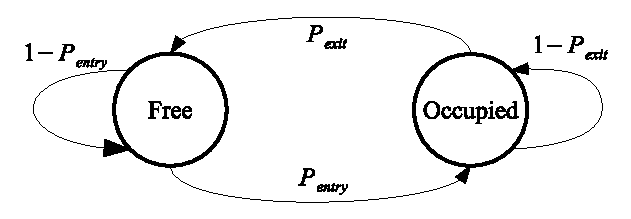
\includegraphics[width=0.7\linewidth]{chapters/mapping_of_dynamic_areas/figures/markow_occupancy_model}
	\caption{Markow chain for occupancy states borrowed from \cite{Saarinen2012}}
	\label{fig:markow_occupancy_model}
\end{figure}

The transitions is modeled as Poisson processes and the rate parameters is estimated as Gamma distributions. This gives in total four variables for each cell, which are used to interpret the type of dynamic for the cell. 

Another method for learning the map dynamics using Hidden Markov Models (HMM) is described by Meyer-Delius et al. \cite{Meyer-Delius2012}. This method uses the same possible states as the IMAC, but as it is a HMM the states are not directly observable thus it is possible to incorporate sensor uncertainty. In order to learn the parameters of the model two methods are used; an offline and an online approach. The offline approach requires storing all observations and then iteratively learn the parameters using the expectation-maximization algorithm. The online version of the parameter learning algorithm, developed by Mongillo and Deneve \cite{Mongillo2008} eliminates the need for storing the whole observation set. Instead only 16 values has to be stored for each cell and the iterative learning can be done online. The online method is capable of handling changing dynamics by using a forget factor. 

A different approach to mapping the dynamics is the Frequency Map Enhancement (FREMEN) proposed by Krajník et al. \cite{Krajnik2014}. This method models the dynamics of each cell by its primary frequency components. 
For prediction of future state the frequencies are reconstructed to a signal, which determines the predicted cell value. 
These uses a limited and constant number of parameters per cell. However, the method also requires the storage of time spans where the prediction went wrong in order to determine when a new model is needed. This significantly increases the memory requirements of the method.

With the reconstructed signal it is possible to predict infinitely long out in the future if it object moves with that frequency. 
This is not the case for Markow processes where the predicted probability for being in a state stabilizes on a constant, after many state changes.
There are also disadvantages with the method.
The most prominent comes from the fact, that it is impossible to recover a signal with a frequency lower than the Rayleigh-frequency of $1/T$, where $T$ is the period. 
This demands for storing measurements for the time period in which objects appears, disappears and appears again. This period can everything from hours for vehicles to days or weeks for stocked product parts. 
It might be possible to degrease the amount of stored information by only storing the average taken over periods, but then it is impossible reconstruct objects moving faster than the period which the average is taken. 

The characteristics of the six methods to improve occupancy grid mapping by learning the dynamics of the environment are outlined in table \ref{tab:learners_characteristics}.

\begin{table}[htbp]
    \centering
    \caption{Characteristics of methods to learn dynamics in occupancy grids.}
    \label{tab:learners_characteristics}
    \begin{tabular}{p{2.6cm} | p{1.6cm} | p{4.cm} | p{2.6cm} | p{1.6cm}}
        \toprule
        \textbf{Name} & \textbf{Memory} & \textbf{Dynamic representation} & \textbf{Learning method} & \textbf{Handles dynamics} \\
        \rowcolor[gray]{0.925}
        TOG & High & Time averaged OG & Online batch & Yes \\
        TSM & High & Time  averaged OG & Random sample replacement  & Yes\\
        \rowcolor[gray]{0.925}
        IMAC & Low & Markov parameters & Online iterative & Yes \\
        HMM - Offline & High & Markov parameters & Offline batch  & No \\
        \rowcolor[gray]{0.925} 
        HMM - Online & Low & Markov parameters & Online iterative & Yes \\
        FREMEN & Medium & Frequency components & Online batch & Yes\\
        \bottomrule
    \end{tabular}
\end{table}

\subsection{Methods ability to learn Markow Processes}
The described methods that models dynamic with Markow processes are compared with a simple simulation where a grid cell are occupied by a dynamic obstacle. 
Whether the cell is occupied or free is controlled by a Markow process with $0.9$ probability for entering and $0.2$ probability for exiting the cell. 
The process is observed by an one dimensional range sensor, which can measure too short with a probability of $0.16$, in which case the online-HMM are propagated one step without adding new information and the IMAC is left unchanged.
There is an equal probability for the sensor measuring a range too far, which results in a reading of an empty cell independently of the cell's state. 
Figure \ref{fig:markow_learning} shows that IMAC is unable to converge to the correct state transition probabilities, where as the HMM-online method that incorporate the uncertainties in measurements slowly converges toward them.
The state transitions estimated by IMAC are so far from the actual parameters that they are almost useless for prediction. 
The number of measurements needed for HMM-online to converge is however very large.
Considering that the simulation is setup so that the object has a considerable possibility of moving between each measurement, it will be very time consuming to learn the transition probabilities for obstacles moving at days between.

\begin{figure}[htbp]
    \centering
    \begin{subfigure}[t]{0.45\textwidth}
        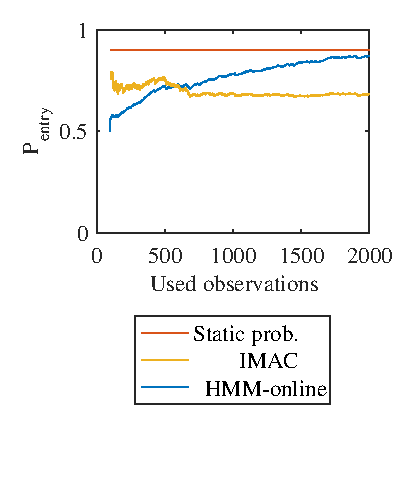
\includegraphics[width=1.0\textwidth]{chapters/mapping_of_dynamic_areas/figures/markow_learn_1d_entry}	
        %\caption{}
        %\label{fig:markow_learn_1d_entry}
    \end{subfigure}
    \begin{subfigure}[t]{0.45\textwidth}
        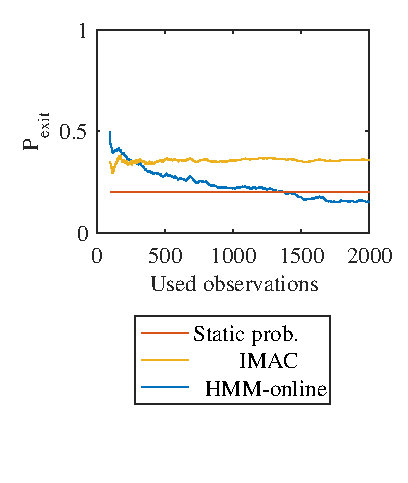
\includegraphics[width=1.0\textwidth]{chapters/mapping_of_dynamic_areas/figures/markow_learn_1d_exit}
        %\caption{}
        %\label{fig:markow_learn_1d_exit}
    \end{subfigure}
    \caption{Learned state transition probabilities compared to the simulated Markow process.}
    \label{fig:markow_learning}
\end{figure}

\section{FreMEn - Predicting future occupancy}
\label{sec:fremen}
The  Frequency Map Enhancement (FreMEn) method models the dynamics of each cell by its primary frequency components. It has successfully been applied to improve mobile robots ability to perform feature-based localization \cite{online_fremen} and topological navigation \cite{fentanes2015}. Here Krajník et al. argues for approximating the appearance and disappearance of obstacles with multiple periodic sinus signals, since people often moves them as part of daily routines. As discussed in section \ref{sec:characteristics_in_industrial_environments} this might also be the case in the industrial environments in focus here. Resent work in \cite{life_long_exploration}, shows how the often violated assumption in FFT about a fixed sampling rate is met by incrementally adding sparse and irregular observations. Where the approach usually uses the number of frequency components(m) that minimizes the difference between predicted states and measurements, it is chosen to use the typical order m=2 \cite{life_long_exploration} for all cells. This will probably decrease the prediction performance, but enables online updates without having to store observations for evaluation.

The online variant of the approach updates the parameters shown in equation \ref{eq:fremen_time} for each new measurement $s(t)$. 
The average occupancy probability $\alpha_0$ models the $0Hz$ signal and is updated with a new measurement online. 
The number of measurements n is incremented. There is one of the complex numbers $\gamma_k$ and $\beta_k$ for each $\omega_k=1/T_k$ . 
$T$ is calculated with equation \ref{eq:fremen_update} for each frequency, where N is the 20 used frequency components and epsilon is the smallest period time, which is one minute here. 
The values of consecutive $T_k$ is close for large values of $k$, which is advantageous if most of the obstacles moves with a period close to $\epsilon$.

\begin{equation}
    T_k = \frac{N \epsilon}{k+1}
    \label{eq:fremen_time}
\end{equation}

The real and imaginary part of $\gamma_k$ and $\beta_k$ are updated as the running average. $\gamma_k$ is the part of the signal with the frequency $2 \pi \omega_k$ and $\beta_k$ is the part of this signal which are modeled by the $0Hz$ component of the signal.

\begin{eqnarray}
&\alpha_0 = \frac{1}{n+1}(n \alpha_0 + s(t)) \nonumber \\ 
&\gamma_k = \frac{1}{n+1}(n \gamma_k + s(t) e^{-j \omega_k t}) \forall \omega_k \in \Omega  \\
&\beta = \frac{1}{n+1}(n \beta_k + \alpha_0 e^{-j \omega_k t}) \forall \omega_k \in \Omega \nonumber \\
&n = n + 1 \nonumber
\label{eq:fremen_update}
\end{eqnarray}

When predicting the state of a cell at time $t$ the signal components are calculated with equation \ref{eq:fremen_freq_component}.

\begin{equation}
    \alpha_k = \gamma_k - \beta_k \forall \omega_k \in \Omega
    \label{eq:fremen_freq_component}
\end{equation}

Then $ \Omega $ is ordered based $ | \alpha_k | $ to enable calculation of equation \ref{eq:fremen_predict} using only the $m$ most prominent frequency components. As previously described, we use two frequency components ($ m=2 $) for each cell.

\begin{equation}
p(t) = \zeta \left( \alpha_0 \sum_{k=1}^{m} |\alpha_k| cos(\omega_k t + arg(\alpha_k))  \right)
\label{eq:fremen_predict}
\end{equation}

The function $\zeta$ clamps the expected probability to a value between zero and one. The $arg$-function returns the angle of the complex number with respect to the x-axis.
The occupancy state at time $t$ is predicted as occupied if $p(t)$ is above $0.5$ and as free otherwise.

\begin{figure}[htbp]
\centering
\includegraphics[width=0.4\linewidth]{chapters/mapping_of_dynamic_areas/figures/simulated_environment}
\caption{Screen shot of Stage simulator showing a MIR 100 robot navigating around obstacles which appears and disappears at fixed intervals.}
\label{fig:simulated_environment}
\end{figure}

The methods ability to predict future occupancy states are evaluated in a Stage simulation where many boxes moves in and out at various and fixed, intervals. 
The robot continuously navigates from the lower left corner that are partly surrounded by walls to the top right corner, while the red and green boxes moves around.
The measurements from the simulated LIDAR are incorporated in a temporary local map using the reduced ideal inverse sensor model update method described in section \ref{sec:reduced_ideal_sensor_model}. 
The update values for the sensor model is reduced to incorporate uncertainties in localization.
For every fifth second a global map of FreMEn cells are updated with \ref{eq:fremen_update} where $s(t)$ is the probability for occupancy in the local map. 
The local map is then cleared and the process continues.

\begin{figure}[htbp]
    \centering
    \begin{subfigure}[t]{0.49\textwidth}
        \includegraphics[width=1.0\textwidth]{chapters/mapping_of_dynamic_areas/figures/fremen_ideal_simulation}	
        \caption{Predicted map without noise.}
        \label{fig:fremen_ideal_sim}
    \end{subfigure}
    \begin{subfigure}[t]{0.49\textwidth}
        \includegraphics[width=1.0\textwidth]{chapters/mapping_of_dynamic_areas/figures/fremen_with_decay_last}
        \caption{Predicted map with realistic sensor and localization noise.}
        \label{fig:fremen_sim_with_noise}
    \end{subfigure}
    \caption{Robot navigating in the map predicted with FreMEn where the the green dots marks ends of LIDAR readings.}
\end{figure}

To evaluate the predictive strength of FreMEn it is used to predict the appearance of obstacles each time a new measurement is added from the local map. 
Figure \ref{fig:fremen_ideal_sim} shows how FreMEn correctly predicts the appearance of many of the obstacles when the robots exact position is used to incorporate exact LIDAR measurements. 
Figure \ref{fig:fremen_avg_miss_with_noise} shows a more realistic simulation with Gaussian noise on LIDAR measurements with a standard deviation of one centimeter and localization using AMCL with a static map representation.
Here some of the obstacles are predicted to have moved while they in fact are still present, as shown in the middle to the right in figure \ref{fig:fremen_avg_miss_with_noise}.

FreMEn's lack of ability to predict future measured obstacles is also apparent in the average correctly predicted observations of obstacles. 
This is shown in figure \ref{fig:fremen_avg_correct_predictions} where the good prediction percent on $74.0\%$ drops to $46.9\%$ with the addition of noise.
From the experiment without noise it is concluded that the learned periodic appearance of obstacles in a grid with FreMEn is useful for predictions.
In the presence of noise the signals within the cells becomes more complicated, and the measurements used for comparison is not always correct.
This, combined with the fact that obstacles placed by humans probably will not move in and out of grid cells so consistently as in this simulation, leads us to believe that the implemented method is not useful for online update of the occupancy grid map used by AMCL.
It might however be possible to alter the method, or combine it with others, to take advantage of the methods ability to predict presence of obstacles many hours after the last observation.
The predicted maps can improve the validness of global paths planned by the robot, but with the rather poor prediction percentage many paths have to be re-planned during navigation. 

\begin{figure}[htbp]
    \centering
    \begin{subfigure}[t]{0.49\textwidth}
        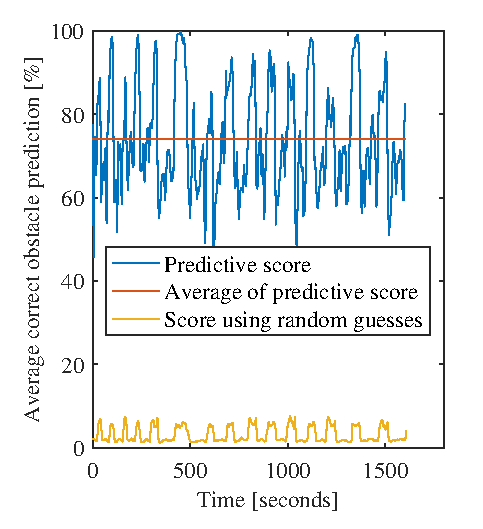
\includegraphics[width=1.0\textwidth]{chapters/mapping_of_dynamic_areas/figures/fremen_avg_miss_no_noise}	
        \caption{Prediction score without noise.}
        \label{fig:fremen_avg_miss_no_noise}
    \end{subfigure}
    \begin{subfigure}[t]{0.49\textwidth}
        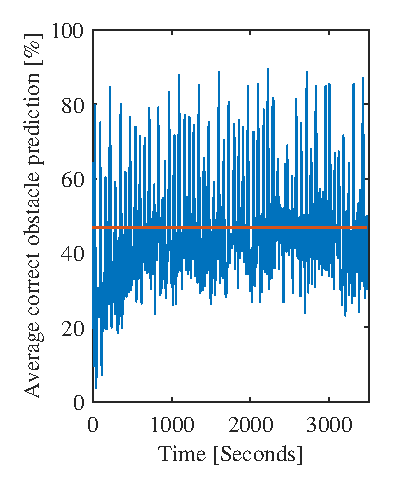
\includegraphics[width=1.0\textwidth]{chapters/mapping_of_dynamic_areas/figures/fremen_avg_miss_with_noise}
        \caption{Prediction score with noise.}
        \label{fig:fremen_avg_miss_with_noise}
    \end{subfigure}
    \caption{Prediction scores for FreMEn defined as the average number of matches between measured and predicted obstacles.}
    \label{fig:fremen_avg_correct_predictions}
\end{figure}

%!TEX root = ../../report.tex
\section{ Probabilistic Input  Markov Chain}
\label{sec:pmac}

\subsection{Developing on independent Markov chains}
The IMAC method considers an observation to be either occupied or free. In the system setup used in this project, however, the input is the probability that a cell is occupied. To use IMAC it is necessary to determine the state of the observation with one or two thresholds. The simplest choice is placing a threshold at $0.5$ rendering everything above as an occupied observation and everything below a free. This approach will make no distinction between an observation of $0.501$ and $0.999$, which both will be considered occupied and contribute equally in the learning process. This is not desirable as the latter measurement contains immensely more information than the former. 
Equating all measurements on the basis that they fall on the same side of a threshold reduces the advantage of taking position and sensor noise into consideration. An example could be a cell observed at a great distance and quite large uncertainty and then later very close by with high confidence in the reading. These two entries into the IMAC learner would carry the same weight. If for instance a reading resulted in a $0.99$ occupancy probability and a following reading produced a $0.49$ occupancy probability, the simple threshold method would register it as an occupied followed by a free and thus adding an event. In reality there is very little evidence for this event happening and if the subsequent reading would again produce a $0.99$ occupancy probability this would introduce even more dynamics disregarding that the evidence is very unsubstantiated. 

Therefore a method of incorporating the uncertainty of the observations and carrying them into the learner is desired. As IMAC is a fast learner of Markov transition probabilities when the observations are very certain, the incorporation of the uncertainties should not hinder that. 

The requirements for the incorporation of the uncertainties are:
\begin{itemize}
	\item Perform as IMAC on perfect input
	\item Avoid low confidence observations counting as much as high confidence
	\item Avoid biasing towards neither static or dynamic
\end{itemize}

The method devised to accomplish the integration of uncertainties is denoted probability input Markov chain (PMAC). As opposed to IMAC the PMAC uses a score rather than a count of a state and event. The state score is calculated as  \(2\cdot|0.5-p_{occ}|\) for the active state which is determined by whether \(p_{occ} > 0.5\) or not. This ensures that if the reading is certain, ie. either 0 or 1 the update will be similar to that of IMAC, and as uncertainty increases the score linearly decreases. The event score is calculated based on how certain the previous state was and how certain the current state is. In order to avoid biasing towards dynamic the maximum, based on the certainty of the previous state, is the average of the consecutive observations in that state. As the average cannot exceed 1 this ensures that in perfect certainty the behavior is equal to that of IMAC. The maximum limit based on the current state is the sum of scores in the current state.

\begin{equation}
IMAC: \lambda = \frac{\#event_{count}}{\#state_{obs}}
\end{equation}

\begin{equation}
PMAC: \lambda = \frac{\Sigma event_{score}}{\Sigma state_{score}}
\label{eq:pmac_lambda}
\end{equation}

\begin{equation}
state_{score}=2 \cdot |0.5-p_{occ}| 
\end{equation}

\begin{equation}
event_{score}=min(\hat{\mu}_{state_{score}}(i-1),state_{score}(i))
\end{equation}

Both the state and event scores behave as IMAC counters when the certainty is perfect, thus fulfilling the first requirement. The second requirement is achieved by the state score scaling with the occupancy probability distance from $0.5$, and the event score basing its value on the state score. Basing the state score on the distance from $0.5$ helps to avoid skewing the result towards static. Another possible scoring could be the probability for occupied and free respectively: 

\begin{equation}
score_{occ} = p_{occ}
\end{equation}
\begin{equation}
score_{free} = 1-p_{occ}
\end{equation}

As the active state is determined by a threshold of $0.5$, this scoring system would always be at least $0.5$, skewing the results. The chosen score better incorporates $0.5$ denoting unknown, thus producing a score of $0$. 

In order to avoid biasing towards dynamic the average of the previous state scores is used. If, instead, the sum had been used, a series of low confidence observations could skew the result. As the state score can be considered $\hat{\mu} \cdot n_{obs}$ the event score will be balanced when using as a maximum value. For instance $5$ observation with an occupancy probability of $0.6$ would each give a score of $0.2$, and the sum would consequently be $1$. Using the sum,  would be $1/1$  thus skewing it towards dynamics. Using the average, the event score is balanced to the state score and produces a more correct value of $0.2/1$. The correctness of this result is evident from the fact that simply counting events and states with IMAC also results in a probability on $\lambda = 1/5$. Hence the correct dynamics is estimated with PMAC and the parameters are only updated according to the confidence in the used observations.

\subsection{PMAC in action - an example}
Figure \ref{fig:state_scores_explained} shows an example of some observation, their occupied probabilities $p_{occ}$ and the subsequent state score. On the score plot the average of sequential observation in the same state are shown as green lines. This sets a maximum limit on the size of the subsequent event score. To demonstrate the workings of PMAC these observations are used as input to the PMAC learner in the following. 

\begin{figure} [htbp]
    \centering
    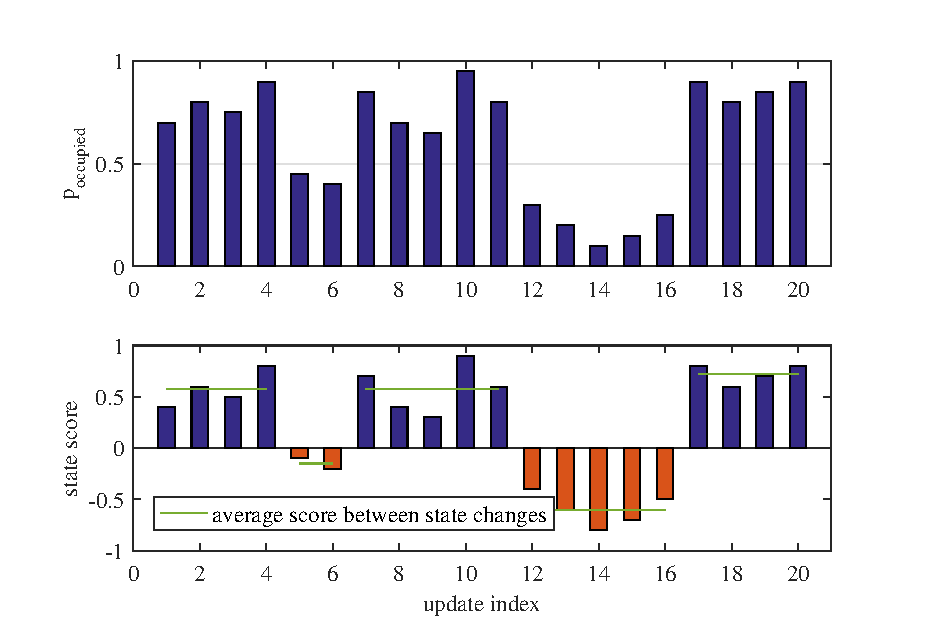
\includegraphics[scale=1]{chapters/mapping_of_dynamic_areas/figures/state_scores_explained}
    \caption{Artificial example of occupancy probabilities used to learn dynamics.}
    \label{fig:state_scores_explained}
\end{figure}

From the state scores in figure \ref{fig:state_scores_explained} it is seen that from index 0 to 11, the situation starts as occupied with quite confident readings. Then $2$ more uncertain reading showing free occurs before confident readings of occupied are again received. The effect of this on the exit is shown in figure \ref{fig:pmac_exit_explained}. The sum of occupied scores increases steadily from index $0$ to $11$, while the event sum increases a comparatively small amount. However it is clearly visible on the exit  value as it is the first observations and both sums are initialized to the smallest possible non-zero value. This initialization is chosen in order to avoid dividing by $0$ and minimizing the effect of the initialization on the result. The effects of this initialization is clearly visible in figure \ref{fig:pmac_entry_explained}, that shows the scores and values for the entry. The entry value is $1$, as the initial values causes, but as soon as input is received their effect is suppressed.

\begin{figure}[htbp]
\centering
\includegraphics[scale=1]{chapters/mapping_of_dynamic_areas/figures/pmac_exit_explained}
\caption{Evolution of parameters used to estimate dynamics with the data shown in figure \ref{fig:state_scores_explained}.}
\label{fig:pmac_exit_explained}
\end{figure}

The observations from index $7$ to $20$ constitutes more certain changes in the state and thus carry more information which can be seen in the sums of especially the free score and entry event score. 

\begin{figure}[htbp]
    \centering
    \includegraphics[scale=1]{chapters/mapping_of_dynamic_areas/figures/pmac_entry_explained}
    \caption{Evolution of parameters used to estimate dynamics with the data shown in figure \ref{fig:state_scores_explained}.}
    \label{fig:pmac_entry_explained}
\end{figure}

\todo{Write about improved pmac handling noise problem}

\begin{figure}[htbp]
\centering
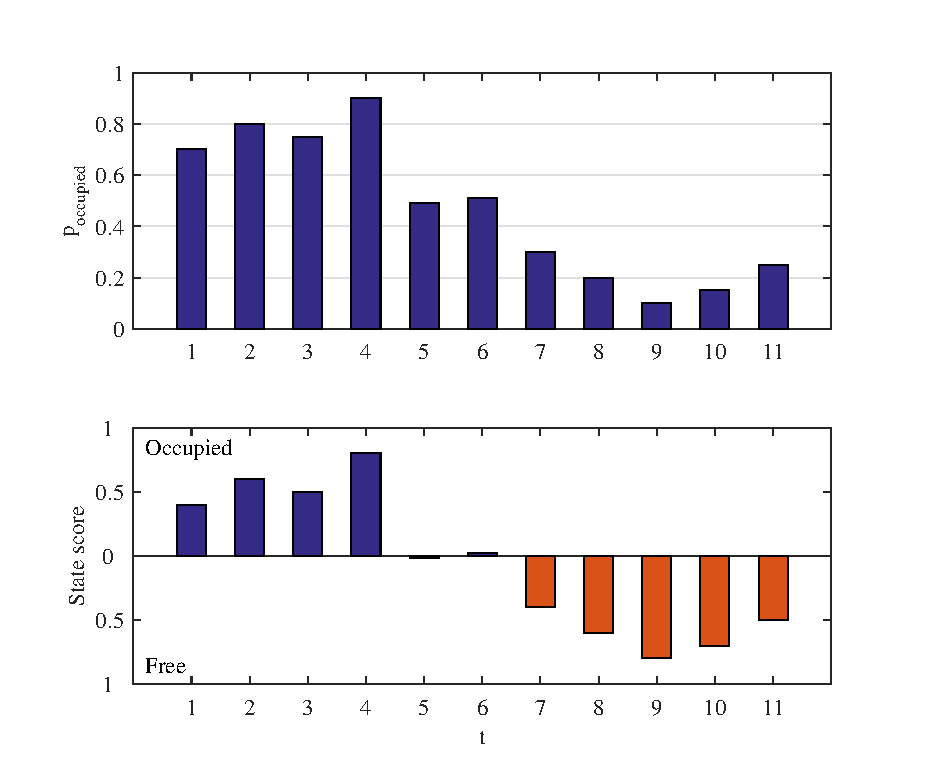
\includegraphics[scale=1]{chapters/mapping_of_dynamic_areas/figures/pmac_noise_problem_case}
\caption{}
\label{fig:pmac_noise_problem_case}
\end{figure}


\begin{figure}[htbp]
    \centering
    \includegraphics[scale=1]{chapters/mapping_of_dynamic_areas/figures/visualization_of_advantage_long_term_average}
    \caption{}
    \label{fig:visualization_of_advantage_long_term_average}
\end{figure}

%INSERT ENTRY FIGURE



Disucussion on underlying Markov model -> Accuracy, Realism

\subsection{Initializing the dynamic map}
As the dynamic map is the result of a learning process it will not contain any information from the onset. 
This might be a problem if the localization and navigation systems are relying on the results to perform their tasks.
To handle this, but also to guide the dynamic map it is possible to initialize the PMAC parameters. 
This could be done by what has previously been learned by the PMAC or by a static map.
The initialization value of the PMAC parameters should be set according to the desired output, considering the interpretation, and  the confidence in the initial map.
If the confidence is high in the obstacles of the initializing map, giving the cells in the dynamic map a strong initialization helps ensure that small errors will have less effect. 
The same principles go for the free areas but it is likely might become obstructed at some point so initializing them too heavily might reduce the usefulness of the dynamic learner.
Three different types of initialization is available from a static map; free, occupied and unknown.
Each type can have different user-defined initialization values in order to accommodate various use-cases.  

%!TEX root = ../../report.tex
\section{Summary}


\begin{figure}[htbp]
	\centering
	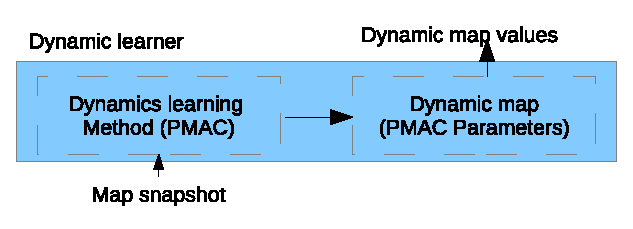
\includegraphics[scale=1]{chapters/mapping_of_dynamic_areas/figures/dynamic_detail.eps}
	\caption{The static mapping in the dynamic mapping system}
	\label{fig:dynamic_learner_detail}
\end{figure}




%!TEX root = ../../report.tex
\chapter{Problem analysis}
\begin{figure}
	\centering
	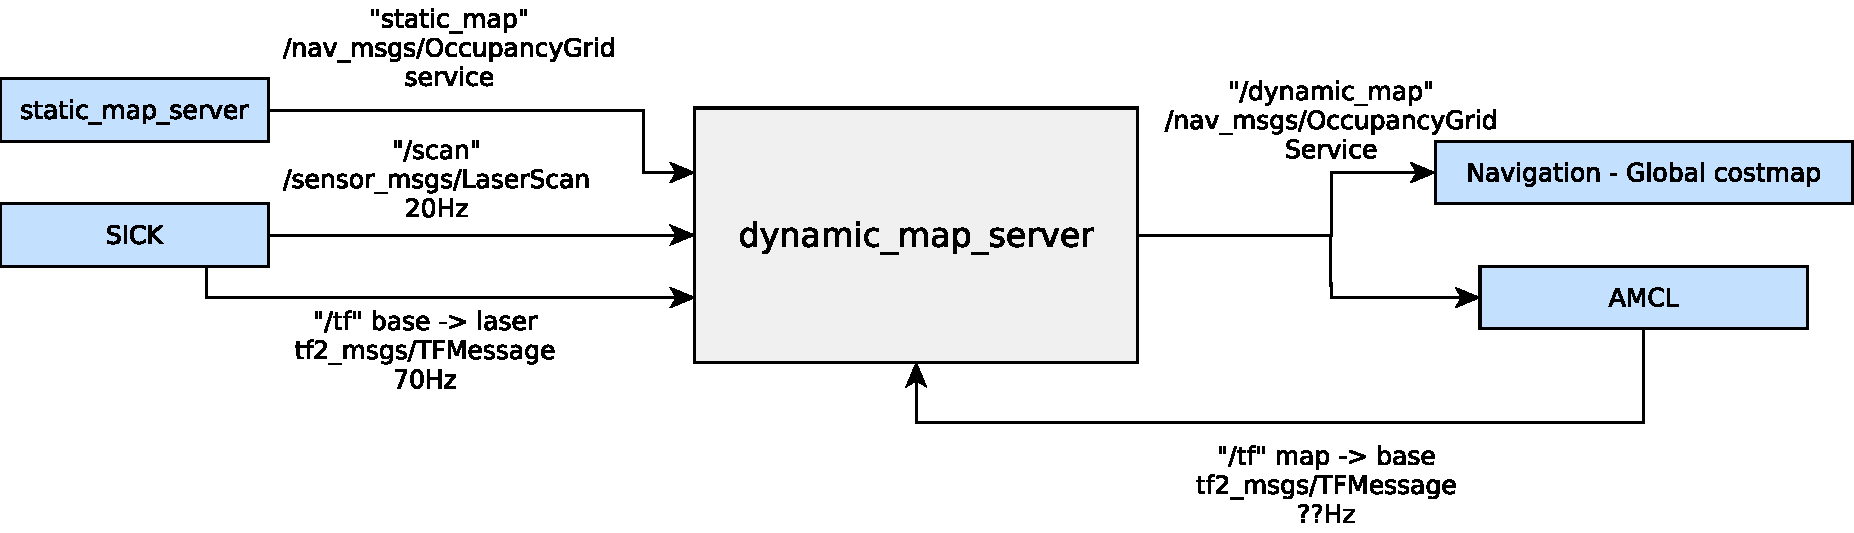
\includegraphics[width=0.6\linewidth]{figures/dynamic_map_mir_interface}
	\caption{Crossing point determined using P4P and an offset from the QR tag in its frame.}
	\label{fig:dyn_map}
\end{figure}
%!TEX root = ../../report.tex
\chapter{Evaluation}
\label{chapter:evaluation}
This chapter evaluates the designed Dynamic mapping system's ability to provide superior navigation and localization by using the observed dynamic behavior of obstacles.
Specifically the following aim is considered:

\begin{enumerate}
    \setcounter{enumi}{3}
    \item Integration and evaluation on the MiR-100 platform
\end{enumerate}

%!TEX root = ../../report.tex
\section{Learning Markov Parameters for Dynamic Obstacles}
\label{sec:learning_markov_evaluation}

\begin{figure}[htbp]
    \begin{subfigure}[t]{0.7\textwidth}	
        \centering	
        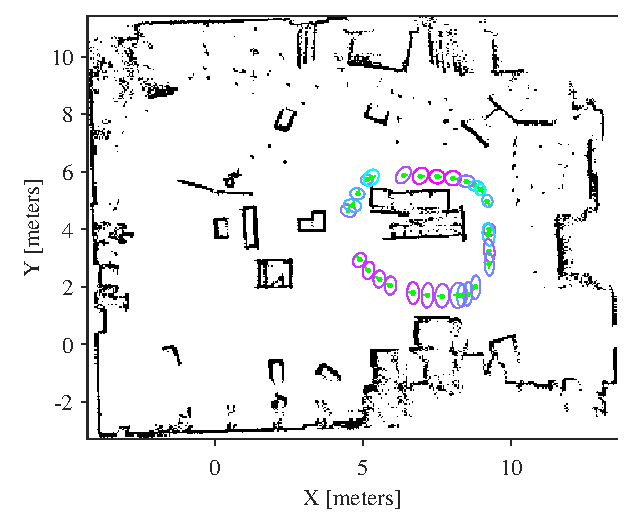
\includegraphics[scale=1.0]{chapters/evaluation/figures/flexlab_path_with_covariance_with_initial_box_positions}
        \end{subfigure}
        \begin{subfigure}[t]{0.2\textwidth}
            \centering
            \includegraphics[scale=1.0]{chapters/evaluation/figures/flexlab_path_with_covariance_bar-crop}
        \end{subfigure}
        \caption{Covariances estimated by AMCL, superimposed on the map with boxes in initial position, shown with contours marking one standard deviation around the robot's estimated pose(green).}
        \label{fig:flexlab_path_with_covariance_first_location_map}
\end{figure}

\begin{figure}[htbp]
    \begin{subfigure}[t]{0.7\textwidth}	
        \centering	
        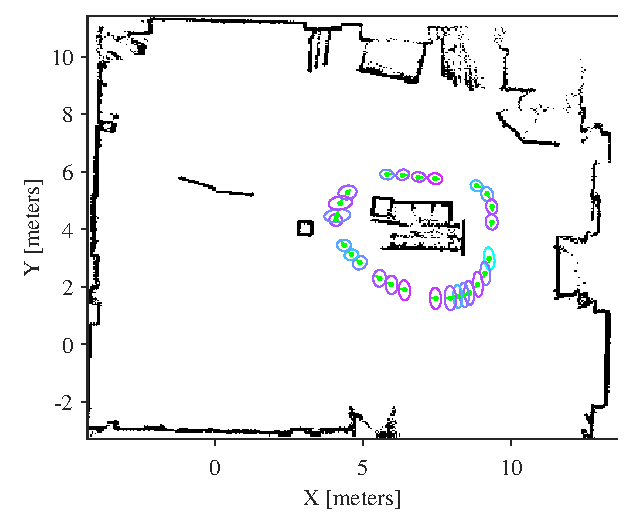
\includegraphics[scale=1.0]{chapters/evaluation/figures/flexlab_path_with_covariance_with_cleaned_map}
    \end{subfigure}
    \begin{subfigure}[t]{0.2\textwidth}
        \centering
        \includegraphics[scale=1.0]{chapters/evaluation/figures/flexlab_path_with_covariance_bar-crop}
    \end{subfigure}
    \caption{Covariances estimated by AMCL, superimposed on the used static map, shown with contours marking one standard deviation around the robot's estimated pose(green).}
    \label{fig:flexlab_path_with_covariance_with_cleaned_map}
\end{figure}

\begin{figure}
\centering
\includegraphics[scale=1.3]{chapters/evaluation/figures/cells_used_for_evaluation_with_identification}
\caption{}
\label{fig:cells_used_for_evaluation_with_identification}
\end{figure}
\begin{figure}
\centering
\includegraphics[scale=1]{chapters/evaluation/figures/compare_learned_markov_entry}
\caption{}
\label{fig:compare_learned_markov_entry}
\end{figure}
\begin{figure}
\centering
\includegraphics[scale=1]{chapters/evaluation/figures/compare_learned_markov_exit}
\caption{}
\label{fig:compare_learned_markov_exit}
\end{figure}




%!TEX root = ../../report.tex

\subsection{Predicting with Markov model}

A use for the dynamic information of a cell is to improve the prediction of the occupancy of a cell. The prediction mechanism used with PMAC is based on an estimated occupancy value. This value is determined through the update-predict method described in section \vref{sec:cost_interpretation_path_planning}. 
In order to demonstrate the prediction, it has been used on the obstacles. The predict error score is calculated by equation \ref{eq:predict_error_score}. This is calculated for a region of interest around the obstacle position. The number of cells used in the calculation is the number of cell in the region for which the new observation has information. 

\begin{equation}
	Error_{score} = \frac{\sum\limits_{i=1}^{n_{cells}} (p_{predict}(i)-p_{observation}(i))^2}{n_{cells}}
	\label{eq:predict_error_score}
\end{equation} 

In the test only one in every 5 observations were used in the update of the current estimate in order to allow the prediction to engage. All observations were, however, used in the learning of Markov parameters. Figure \ref{fig:markov_predict_obst_2} shows the resulting score for PMAC and a simple previous prediction. The previous predictor uses the last observation as predictor, with the same one in five observations added. The score values are rather small due to the fact that the region of interest also contains static free cells which neither predictor has any trouble with. As PMAC is not initialized with any information on the dynamics these are learned through the observations. 
It is seen that the PMAC predictor does a better job at predicting the occupancy state for this obstacle. The effect of using the PMAC will vary for different obstacles. For the obstacles with low transition probabilities using the previous observation as predictor can be a good approximation and can outperform PMAC, especially if PMAC has not learned  accurate Markov parameters.  

\begin{figure}[htbp]
	\centering
	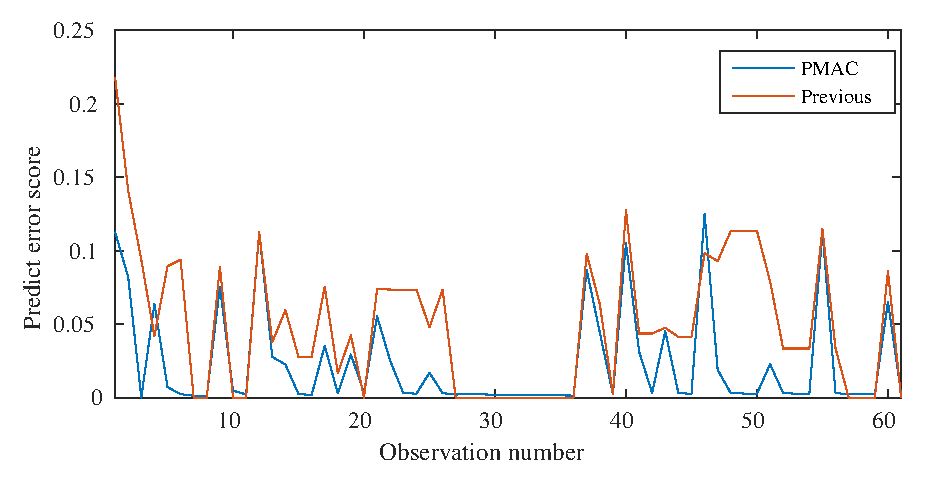
\includegraphics[scale=1]{chapters/evaluation/figures/markov_predict_figs/obstacle2_low.eps}
	\caption{Predict error score for obstacle number 2}
	\label{fig:markov_predict_obst_2}
	
\end{figure}

%!TEX root = ../../report.tex
\section{Monte Carlo Localization with Dynamic Map Representation}
\label{sec:amcl_dyn_map}
The effect of performing localization with AMCL on an updated map representation in the form of the costmap described in section \ref{sec:localzation_feature_map} is evaluated by comparing the estimated pose covariances with the ones achieved when using a static map representation. 
The sizes of the elements of the covariance matrix indicates the certainty of the estimated pose of the robot with respect to the map frame. 
Larger values is evidence for an uncertain pose estimation. Hence the estimated covariance do not indicate how accurate the location estimate is, but how widely spread the particles is. 
It can happen that AMCL is very certain on a wrong position. 

The test setup evaluates a situation where a mobile robot navigates in an area for some time, then it moves away and comes back to a changed environment and navigates there for the same amount of time. 
This is repeated for four times using both a static map representation and a map that is adapted to the changes using the Dynamic mapping system. 

\subsection{Industrial Test Environment}
The evaluation is performed on the MiR-100 robot with the software version 1.5.1. It was performed in Robolab at SDU, which is similar to an industrial environments. Initially the environment was mapped with the Hector SLAM algorithm contained in the MIR software. 
Afterwards, small obstacles which might be moved during the evaluation was removed.
The generated map is shown in figure \ref{fig:Robolab1_clean_with_cam}, where the approximate pose of the camera when taking the images shown in figure \ref{fig:robolab_mayhem} is indicated. 
The camera is positioned on the first floor and tilted.

\begin{figure}[tbph]
	\centering
	\includegraphics[width=0.7\linewidth]{chapters/evaluation/figures/Robolab1_clean_with_cam}
	\caption{The static map used by AMCL with indication of the camera's pose when taking the images in figure \ref{fig:robolab_mayhem}.}
	\label{fig:Robolab1_clean_with_cam}
\end{figure}

The test was performed by letting the robot navigate around the obstacles located central in the room continually for 25 minutes two times in four different environments. 
For each of the environments the robot performed localization on the static map in figure \ref{fig:Robolab1_clean_with_cam} and with a map constructed by the Dynamic mapping system for 25 minutes. 
The Dynamic mapping system incorporates the information collected in the previous test runs.
The first updated map is created using the data collected using the static map representation and the second also incorporates the data collected when localizing with the previous dynamic map. 
The third also incorporates the data collected in the previous experiment when localizing with a dynamic map and so on for the two consecutive environments.

\begin{figure}[htbp]
	\begin{subfigure}[t]{0.499\textwidth}	
		\centering	
		\includegraphics[width=1\textwidth]{chapters/evaluation/figures/mayhem_robolab1}
		\caption{First environment}
		\label{fig:location_environment1}
	\end{subfigure}
	\begin{subfigure}[t]{0.499\textwidth}
		\centering
		\includegraphics[width=1\textwidth]{chapters/evaluation/figures/mayhem_robolab2}
		\caption{Second environment}
		\label{fig:location_environment2}
	\end{subfigure}
	\begin{subfigure}[t]{0.499\textwidth}
		\centering
		\includegraphics[width=1\textwidth]{chapters/evaluation/figures/mayhem_robolab3}
		\caption{Third environment}
		\label{fig:location_environment3}
	\end{subfigure}
	\begin{subfigure}[t]{0.499\textwidth}
		\centering
		\includegraphics[width=1\textwidth]{chapters/evaluation/figures/mayhem_robolab4}
		\caption{Fourth environment}
		\label{fig:location_environment4}
	\end{subfigure}
	\caption{Robolab at SDU technical college with different positions of obstacles.}
	\label{fig:robolab_mayhem}
\end{figure}

In the first environment shown in figure \ref{fig:location_environment1} a table was tilted, eight cardboard boxes and a whiteboard was placed. 
In the second environment shown in figure \ref{fig:location_environment2}, two of the boxes was moved closer, one more table and whiteboard was flipped, and a pallet was moved. 
In the third environments \ref{fig:location_environment3} even more changes are introduced in the form of tilted chairs and a pallet. 
In the forth environment shown in figure \ref{fig:location_environment4} some of the boxes are moved and a whiteboard is moved out of sight. 
This results in fewer changes to the environment since the map was created than in the third environment.

\subsection{Estimation Uncertainty with Dynamic Map Representation}
During navigation the covariance and robot pose, estimated by AMCL is logged. 
The covariances in positions are ignored here to keep the data analysis simple while still enabling a comparison of the estimations achieved while using a static- and dynamic map.
\todo{Bad argument}

Figure \ref{fig:location_data_angle} shows the estimated standard deviation on the estimated orientation of the robot while navigating with a static- and dynamic map representation in the four different environments.
It shows that the estimation variates less when using a dynamic map representation.
In the first environment the estimated deviation is mostly smaller when using a dynamic map representation, but during a short time of every cycle of moving around the obstacle, it is much larger. 
While the lowest estimated deviation while using a static map is only slightly higher in the other environments, it is still occasionally very large, whereas it remains rather constant while using a dynamic map representation. 
From figure \ref{fig:location_data_hist_angle} it is evident that the estimation is distributed with a normal distribution.
The one-sided student-T test with unequal variance shows that the estimated standard deviation of the orientation is smaller when using a dynamic map with $p < 0.001$.

\begin{figure}[htbp]
	\begin{subfigure}[t]{1\textwidth}	
		\centering	
		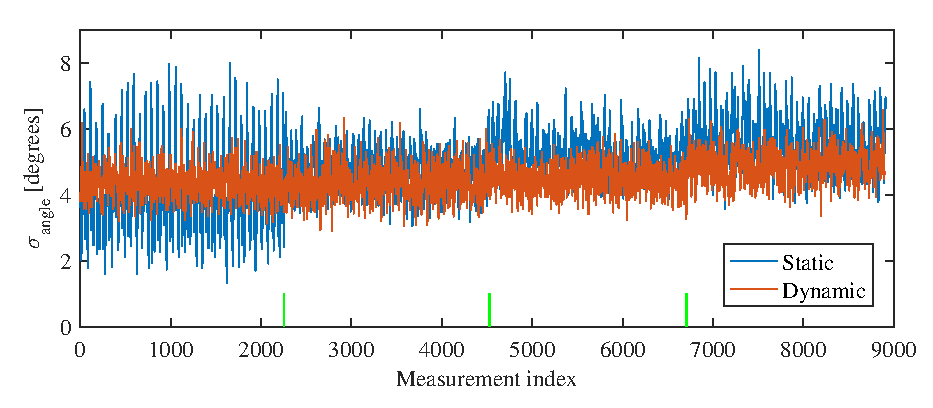
\includegraphics[scale=1.0]{chapters/evaluation/figures/location_data_angle}
		\caption{Estimated standard deviation on the estimated orientation during the four different experiments. The green lines in the figure indicates changes from one experiment to the next.}
		\label{fig:location_data_angle}
	\end{subfigure}
	\begin{subfigure}[t]{1\textwidth}
		\centering
		\includegraphics[scale=1.0]{chapters/evaluation/figures/location_data_hist_angle-crop}
		\caption{Histogram of the estimated standard deviation of the orientation estimate.}
		\label{fig:location_data_hist_angle}
	\end{subfigure}
	\caption{Estimated standard deviation of the estimated orientation while navigating in the four different environments.}
	\label{fig:location_angle_evaluation}
\end{figure}

Figure \ref{fig:location_data_x} and \ref{fig:location_data_y} shows the estimated standard deviation of the estimated x- and y position receptively, while navigating with a static- and dynamic map in the four different environments. 
It is clear that the estimated deviation varies less when using a dynamic map representation.
Where the estimated deviation remains almost constant throughout the four experiments, it is often much larger when using a static map representation. 
These tendencies are especially profound in the last environment in the x direction and in the first in the y direction. 
The estimations are not normal distributed as seen in figure \ref{fig:location_data_hist_x} and \ref{fig:location_data_hist_y}.
While the histograms over the position deviations indicates that the estimated deviation is smaller when using a dynamic map representation the median of it is not statistical significant smaller. This is evident from the one-sided Wilcoxon Rang-Sum test.
\begin{figure}[htbp]
	\begin{subfigure}[t]{1\textwidth}	
		\centering	
		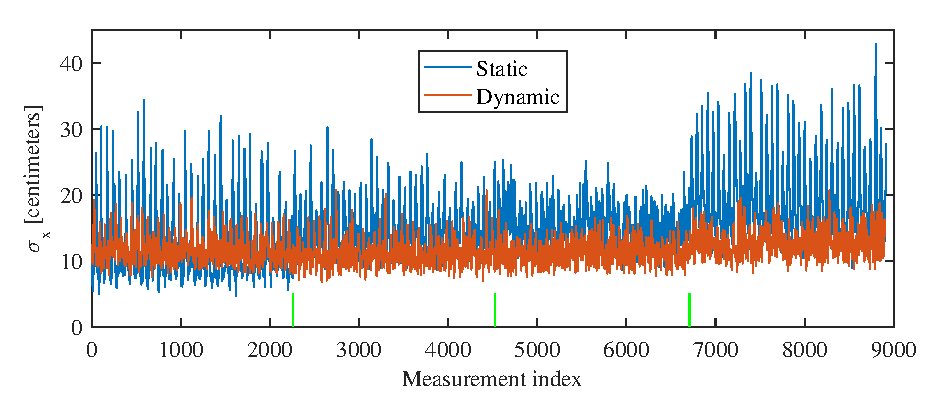
\includegraphics[scale=1.0]{chapters/evaluation/figures/location_data_x}	
		\caption{Estimated standard deviation on the estimated x-position during the four different experiments. The green lines in the figure indicates changes from one experiment to the next.}
		\label{fig:location_data_x}
	\end{subfigure}
	
	\begin{subfigure}[t]{1\textwidth}
		\centering
		\includegraphics[scale=1.0]{chapters/evaluation/figures/location_data_hist_x-crop}
		\caption{Histogram of the estimated standard deviation of the x-position estimate.}
		\label{fig:location_data_hist_x}
	\end{subfigure}
	\caption{Estimated standard deviation of the estimated x-position while navigating in the four different environments.}
	\label{fig:location_x_evaluation}
\end{figure}

\begin{figure}[htbp]
	\begin{subfigure}[t]{1\textwidth}	
		\centering	
		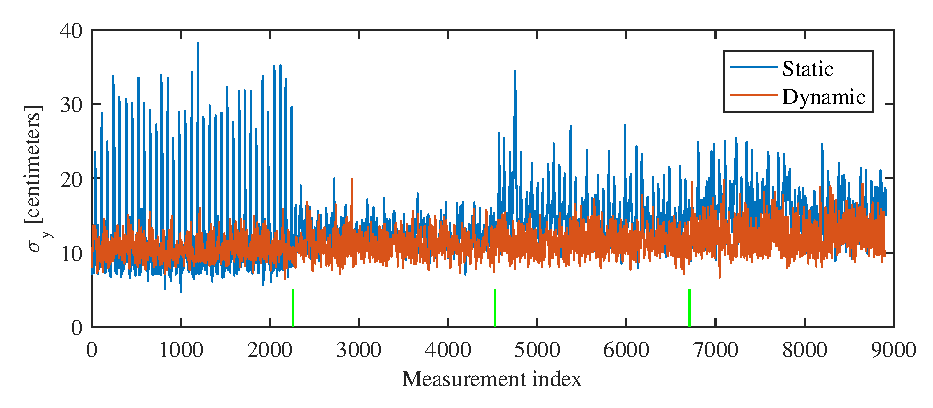
\includegraphics[scale=1.0]{chapters/evaluation/figures/location_data_y}	
		\caption{Estimated standard deviation on the estimated y-position during the four different experiments. The green lines in the figure indicates changes from one experiment to the next.}
		\label{fig:location_data_y}
	\end{subfigure}
	
	\begin{subfigure}[t]{1\textwidth}
		\centering
		\includegraphics[scale=1.0]{chapters/evaluation/figures/location_data_hist_y-crop}
		\caption{Histogram of the estimated standard deviation of the y-position estimate.}
		\label{fig:location_data_hist_y}
	\end{subfigure}
	\caption{Estimated standard deviation of the estimated y-position while navigating in the four different environments.}
	\label{fig:location_y_evaluation}
\end{figure}

\subsection{Jumps in Position Estimation with Dynamic Map Representation}
The AMCL localizations with a static map makes large jumps between estimated localization when the robot is located close to the box standing by the net furthest from the camera in figure \ref{fig:robolab_mayhem}. 
In all four environments the estimated position suddenly jumps to be much closer to the net. 
The effect is probably due to multiple consecutive laser scans hitting the boxes, but scoring the particles as if they had hit the net behind them.
Figure \ref{fig:amcl_covariance_static1} shows this jump in the estimated position of the robot superimposed on the map as it is observed by the robot.
Considering that the robot cannot physically be located so close to the boxes, the correct robot pose is more closely estimated with the dynamic map representation as shown in figure \ref{fig:amcl_covariance_dynamic1}.
The estimated robot pose is superimposed on the dynamic map representation used by AMCL.

\begin{figure}[htbp]
	\centering
	\begin{subfigure}[t]{0.55\textwidth}
		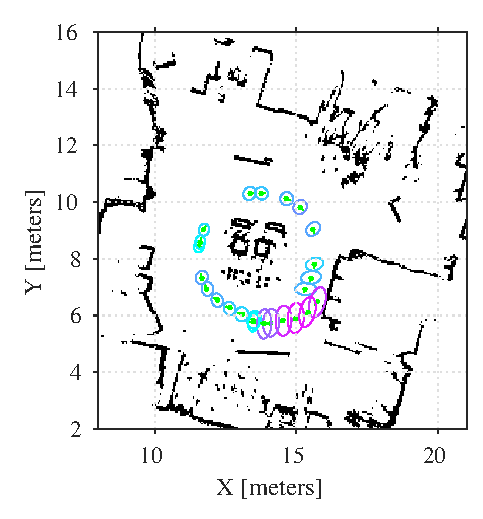
\includegraphics[scale=1.0]{chapters/evaluation/figures/localization_static_map1}		
	\end{subfigure}
	\begin{subfigure}[t]{0.2\textwidth}
		\raisebox{1cm}{\includegraphics[scale=1.0]{chapters/evaluation/figures/localization_std_color_bar-crop}}
	\end{subfigure}
	\caption{Covariances estimated by AMCL with a static map in the first test environment shown with contours marking one standard deviation around the robot's estimated pose(green).}
    \label{fig:amcl_covariance_static1}
\end{figure}

The estimated deviation is generally higher in the third environment where fewer of the laser scans match with the static map representation as shown in figure \ref{fig:amcl_covariance_dynamic1}. 
The reason for the fewer matches is that the dynamic obstacles block for the light beams. 
When using the dynamic map representation shown in figure \ref{fig:amcl_covariance_static3} the estimated deviation is smaller, since the obstacles that has consistently been present while navigating with the dynamic map in the first and second environment.
By comparing the maps in figure  \ref{fig:amcl_covariance_static1} and \ref{fig:amcl_covariance_static3} it is evident that only the obstacles that was present in the first environment is considered static enough to be included in the dynamic map in figure \ref{fig:amcl_covariance_dynamic3}.

\begin{figure}[htbp]
	\centering
	\begin{subfigure}[t]{0.55\textwidth}
		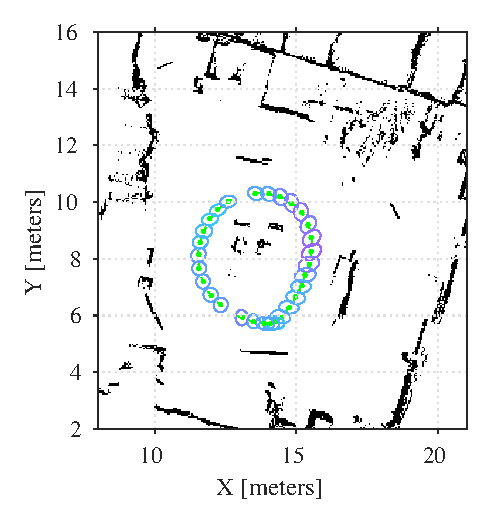
\includegraphics[scale=1.0]{chapters/evaluation/figures/localization_dynamic_map1}		
	\end{subfigure}
	\begin{subfigure}[t]{0.2\textwidth}
		\raisebox{1cm}{\includegraphics[scale=1.0]{chapters/evaluation/figures/localization_std_color_bar-crop}}
	\end{subfigure}
	\caption{Covariances estimated by AMCL with a dynamic map in the first test environment shown with contours marking one standard deviation around the robot's estimated pose(green).}
	\label{fig:amcl_covariance_dynamic1}
\end{figure}

\begin{figure}[htbp]
	\centering
	\begin{subfigure}[t]{0.55\textwidth}
		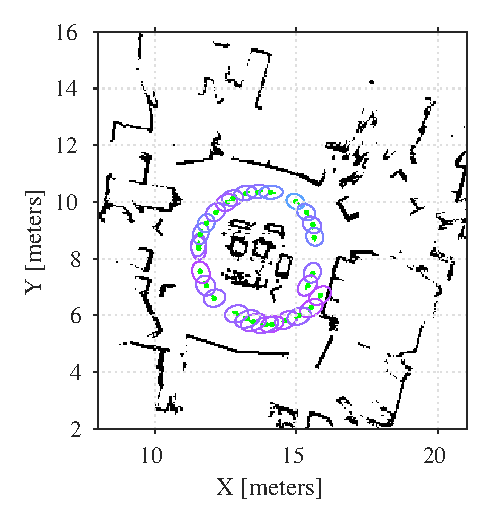
\includegraphics[scale=1.0]{chapters/evaluation/figures/localization_static_map3}		
	\end{subfigure}
	\begin{subfigure}[t]{0.2\textwidth}
		\raisebox{1.15cm}{\includegraphics[scale=1.0]{chapters/evaluation/figures/localization_std_color_bar-crop}}
	\end{subfigure}
	\caption{Covariances estimated by AMCL with a static map in the third test environment shown with contours marking one standard deviation around the robot's estimated pose(green).}
    \label{fig:amcl_covariance_static3}
\end{figure}

\begin{figure}[htbp]
	\centering
	\begin{subfigure}[t]{0.55\textwidth}
		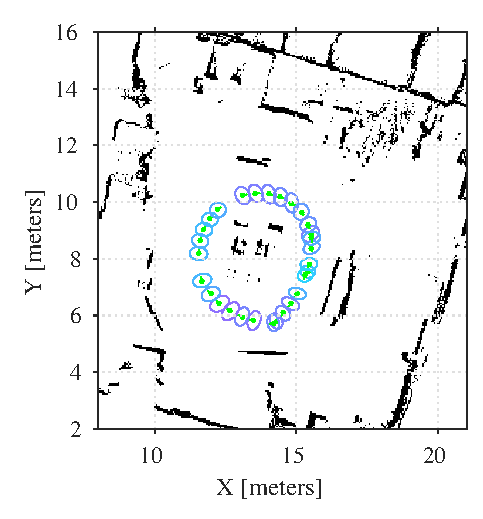
\includegraphics[scale=1.0]{chapters/evaluation/figures/localization_dynamic_map3}		
	\end{subfigure}
	\begin{subfigure}[t]{0.2\textwidth}
		\raisebox{1.15cm}{\includegraphics[scale=1.0]{chapters/evaluation/figures/localization_std_color_bar-crop}}
	\end{subfigure}
	
	\caption{Covariances estimated by AMCL with a dynamic map in the third test environment shown with contours marking one standard deviation around the robot's estimated pose(green).}
    \label{fig:amcl_covariance_dynamic3}
\end{figure}

%!TEX root = ../../report.tex
\section{Accuracy and Precision of Localization with Dynamic Map}
The effects of using a map generated with the Dynamic mapping system for localization is evaluated on the MiR-100.
The localization error is evaluated by comparing the robots estimated pose with the actual pose measured with a camera. 

\subsection{Test setup} 
The robot navigated, with the planner in the MIR software along the paths shown in figure  \ref{fig:amcl_covariance_static1} using a both a adjusted static and a dynamic map, for one hour each.
The software used to navigate and locate is based on the MIR software version 1.5.1. 
The robot stops in the lower left corner on the path during each cycle, where a camera is mounted almost parallel to and approximately $3.3$ meters above the floor.

\begin{figure}[htbp]
    \centering
    \begin{subfigure}[t]{0.45\textwidth}
        \includegraphics[scale=1]{chapters/evaluation/figures/localization_on_adjusted_static_map}
        \caption{Adjusted map representation superimposed with uncertainties estimated while using it.}
        \label{fig:localization_on_adjusted}
    \end{subfigure}
    \hspace{2mm}
    \begin{subfigure}[t]{0.45\textwidth}
        \includegraphics[scale=1]{chapters/evaluation/figures/localization_on_ground_truth__map}
        \caption{SLAM'ed map superimposed with uncertainties estimated while using the Dynamic Mapper System.}
        \label{fig:simulated_true_map}
    \end{subfigure}
    \begin{subfigure}[t]{1\textwidth}
        \centering
        \includegraphics[scale=1.0]{chapters/evaluation/figures/localization_bar-crop}
    \end{subfigure}
    \caption{The path followed by the MiR-100 to a stop in the top left corner under a camera.}
    \label{fig:test_map_setup}
\end{figure}

The adjusted map shown in figure \ref{fig:localization_on_adjusted} is edited manually to simulate changes in the environment. These changes could symbolize pallets with product parts being moved. 
The obstacles located to the left, above and below the robot, has been moved approximately $60$ centimeters away from the robot's path.
Furthermore the pallet the robot drives around is moved approximately $45cm$ towards the top left corner.
Obstacles to the left of the robot's path is moved about $25cm$ towards it.

The map shown in green in figure \ref{fig:static_classified_localization_test-crop} indicates obstacles that are classified as static using the Dynamic mapping system.
The systems learns from data collected for an hour, where AMCL is used for localization with the adjusted map.
It is only the cells that are observed by the robot during the evaluation that are learned. 
The rest originates from a initialization with the map in figure \ref{fig:localization_on_adjusted}.
Figure \ref{fig:static_classified_localization_test-crop} shows that the static obstacles are primarily learned correctly in the regions where the estimation uncertainty in figure \ref{fig:localization_on_adjusted} is low.

\begin{figure}
    \centering
    \includegraphics[scale=1]{chapters/evaluation/figures/static_classified_localization_test-crop}
    \caption{Static obstacles learned with the Dynamic mapping system compared with the SLAM'ed map.}
    \label{fig:static_classified_localization_test-crop}
\end{figure}

On top of the robot a chessboard marker is placed such that the marker frame is positioned on top of the robots base link frame between the wheels.
The chessboard marker is detected using the MATLAB function detectCheckerboardPoints, which detects it with subpixel accuracy \cite{matlab_detect_checkerboard}.
Considering that one pixel is measured to be equivalent to a distance of $2.8mm$ on top of the robot, it is evident that the pose of the marker is detected rather accurate.
The pose of the chessboard on the robot relative to a camera located above it is detected using MATLAB with the extrinsics function \cite{matlab_extrinsics} after calibrating the camera with MATLAB's Camera Calibrator App  \cite{camera_calibrator_app}. 
The camera calibration resulted in a mean reprojection error taken over all the images of $0.15pixels$, which is definitely acceptable.

\subsection{Results}
The estimated poses of the robot while localizing on a static or dynamic map are compared on how much they differ from the pose detected with the camera.
In order to compare the robot pose estimated by AMCL with the pose estimated by the camera. The pose of the marker relative to the camera was converted to represent the pose of the robot.

An estimate of the localization error for each of the poses is obtained by subtracting the accurate robot pose estimated by the camera from the pose estimated by AMCL.
Figure \ref{fig:precision_test_positions} shows the deviation in position using the dynamic map is less spread, and that the accuracy is much higher.
This is also evident for the euclidean distance of the localization error shown in figure \ref{fig:localization_position_error_distance-crop}. 
It shows a significant lower median of the position error when using the dynamic map, which is confirmed by the one-side Wilcoxon-test with a $p<0.001$.
The mean localization position error is actual $60.0\%$ less when using the dynamic map than with the static map.
Figure \ref{fig:localization_position_error_distance-crop} also shows significant changes in localization precision. 
The standard deviation is actually $70.0\%$ lower when using the dynamic map compared to when using the static.

\begin{figure}
    \centering
    \includegraphics[scale=1]{chapters/evaluation/figures/Localization_position_errors}
    \caption{Deviation in estimated robot position when using a static and dynamic map.}
    \label{fig:precision_test_positions}
\end{figure}

\begin{figure}
    \centering
    \includegraphics[scale=1]{chapters/evaluation/figures/localization_position_error_distance-crop}
    \caption{Euclidean deviation in estimated robot position when using a static and dynamic map.}
    \label{fig:localization_position_error_distance-crop}
\end{figure}

The estimated angle deviates less, as show in figure \ref{fig:precision_test_angles}. 
There is no significant difference in the median angle error when using the dynamic map compared to the static.
The precision of the estimated angle is however significantly smaller when using a dynamic map, as shown by the one-sided F-test for equal variance, which is rejected with $p<0.001$.
The improvement amounts to a $56.7\%$ lower standard deviation when using the dynamic map instead of the static.

The statistics for the localization errors when using a static and dynamic map are summarized in table \ref{tab:localization_errors}. It shows improved accuracy and precision in the position estimation when using a dynamic map. The precision is also radically improved for the orientation estimation, but there is only a small difference in the accuracy.
\begin{figure}
    \centering
    \includegraphics[scale=1]{chapters/evaluation/figures/localization_angle_error-crop}
    \caption{Deviation in estimated robot orientation when using a static and dynamic map.}
    \label{fig:precision_test_angles}
\end{figure}

\begin{table}[htbp]
    \caption{Statistics for localization errors}
    \label{tab:localization_errors}
    \begin{center}
        \begin{tabular}{l c  c  c  c}
            \toprule
            \textbf{Map type} & \textbf{Mean position} & $\boldsymbol{\sigma_{position}}$  & \textbf{Mean angle} & $\boldsymbol{\sigma_{angle}}$\\ 
            \rowcolor[gray]{0.925}
            Dynamic & $7.7cm$ & $2.9cm$ & $0.5^\circ$ & $0.9^\circ$  \\ 
            Static & $19.4cm$ & $9.7cm$ & $0.7^\circ$ & $2.2^\circ$  \\ 	
            \bottomrule
        \end{tabular} 
    \end{center}
\end{table}

\section{Discussion}


\subsection{Ability to Learn Dynamics of environment}
The proposed PMAC methods ability to learn the dynamic behavior was investigated by letting it learn from observations of obstacles moving with a controlled Markov process.
The errors in the estimated Markov parameters when using the PMAC learner described in section \ref{sec:learning_markov_evaluation} most likely stems from unmodeled localization errors and insufficient number of observations. 

The wrong estimates for lambda $\lambda_{entry}$ might be due to the fact that cells near the edges of obstacles are often wrongly observed free when the end of the ray-traced lines are too long due to errors in the estimated robot pose.
When the lines are too short due to localization errors the cells further from the laser in the direction of the line are however not counted up as occupied.
This causes an increase in free count values compared to the ones in the entry event counter, which results in the $\lambda_{entry}$ values being too small.
The estimated $\lambda_{exit}$ do not suffers from this problem and are also better, but the small amount of measurements is simply not sufficient to achieve accurate estimates for all the boxes.

Despite the fact that it cannot be shown that PMAC learns the dynamics of semi-static obstacles fast,
the method is useful to improve prediction of future probability for occupied and location of static obstacles.

\subsection{Prediction of Obstacles Location}
When predicting five minutes out into the future in between updates a better match with the observed observation is achieved when using the proposed predict-update method, than when just predicting with the previously observed probability for occupied.
It should be noted that these results are not general, since the accuracy of the prediction depends on the time between observations and how dynamic the observed obstacle are.

\subsection{Localization with Dynamic Map}
The estimation certainty of the localization performed by AMCL is smaller when using a dynamic map.

Jumps in estimated position to an invalid pose is avoided.

The accuracy and precision of the localization is better when using a dynamic map representation.
The navigation system arrives faster at an accurate pose.




%!TEX root = ../../report.tex
\chapter{Discussion and Conclusion}

Throughout this thesis a system was developed to handle the mapping, learning and representation of dynamic environments.
Specifically the aims of the thesis was:
\begin{enumerate}
	\item Precise mapping of static environments by incorporating sensor and localization noise
	\item Long-term, fast, adaptive map representation of dynamic environments
	\item Improved localization with a continuously adapted map of good features
	\item Integration and evaluation on the MiR-100 platform
\end{enumerate}

\section{Discussion}

 

\subsection{Precise Mapping of Static Environments by Incorporating Sensor and Localization Noise}
Tests and real world observations clearly showed the necessity of taking different noise sources into account. 
The developed method of incorporating noise was by a degradation of the update value for each observation. 
In order to account for the sensor noise the chosen sensor model is a reduced version of the ideal sensor model. 
This sensor model was chosen over the commonly used Elfes model due to its better evaluation scores. 
The Elfes model was developed to account for sensor noise but the localization noise present in the system overshadowed the effect of the sensor noise. 
The Elfes model was also tested with the same localization uncertainty weighting as the reduced ideal model and this improved the results of the Elfes model, but did not surpass the reduced ideal model. 
The simulation that the static mapping comparisons was based on might differ from real world experience due to differences in sensor noise and localization noise. 
The localization system used in the simulation is prior to version 1.5.1. of the MIR software. 
Version 1.5.1. introduced improvements to the localization system which may cause different results. 

\subsection{Long-term, Fast, Adaptive Map Representation of Dynamic Environments}
The representation of the dynamics in the environment is a Markov grid. 
Each cell contains an independent Markov process used to represent the probability that changes in state occur. 
The assumption that the process contained in each grid cell is independent is questionable. 
As most obstacles are larger than one cell it will cover multiple cells which will then enter and exit states together. 
Furthermore cells close to each other will probably have correlating states and changes due to the specific use of an area. 

In order to learn the parameters of the Markov processes the PMAC method was developed. 
This method was based on IMAC but with added incorporation of the static mapper, used in this project. 
The primary difference is the scores used to estimate the probability for a state being observed and a state change occurring.
As the Markov model operates with discrete states, and the Static mapper maps with continues occupancy probabilities, the scores are used to model the probability of a state. 
The probability for the cell being in a certain state now and a different state previously determines the probability for a state change.
The probability for a state change occurring must exist and the state and event scores are used to estimate this.  

The scores were developed to handle observations with widely varying certainty. 
In tests PMAC had mixed results. 
A difference in the accuracy of the two different transition probabilities was observed. 
The cause of the disparity might be an unbalance that stems from the sensor model. 
The sensor will clear multiple cells and only mark one. 
This is due to the model modelling the physical properties of a laser ray. 
The model found to be best at mapping static environments uses balanced values, the values of marking and clearing are equal but with opposite signs. 

\subsection{Improved Localization with a Continuously Adapted Map of Good Features}

In the evaluation test it was seen that the obstacles learned as static occupied helped increase the accuracy and precision of the localization compared to using an imperfect static map. 

A threat to the continued reliability of the dynamic mapping is the possible feedback from bad localization estimates. 
If the localization is consistently wrong in an area the features learned might be offset which could cause further degradation of the pose estimate.
This scenario will partly violate an assumption in the dynamic mapping system. 
It is assumed that the world changes slowly enough to provide reasonably accurate pose estimates until an updated map is provided. 
If the robot only rarely observes areas slower changes might over time cause enough discrepancy between the map and the environment to cause localization failure.
In such cases a full SLAM solution is required.
In industrial settings it is likely that a robot operates along fixed routes or within certain areas. This means that that area of operation will be frequently visited and thus reduce the risk of these failures.

Even if a local area has not been closely mapped for some time, if it is within sight areas where updated maps are available this can improve the localization. 
This was seen in the localization test where better localization was achieved by using the learned map, even though the map was learned under imprecise localization.

\section{Conclusion}
The overall aim of the thesis is to develop a mapping system capable of maintaining a consistent map of a changing environment, which facilitates improved navigation of mobile robots.
The designed Dynamic mapping system achieves this by representing dynamics learned from LIDAR measurements while considering the associated uncertainties.
By separating system into the components; Static mapper, Dynamic learner and Cost interpretor, it is possible to develop them based on widely used principles. 
The components are implemented to enable easy exchange for different requirements, while maintaining a general interface.

Previous methods for mapping dynamics are often based on a full SLAM algorithm, which requires extended amount of resources and can result in suboptimal maps due to problems with data association.
Instead we propose to separate the mapping from localization, which is viable due to AMCL's ability to handle moderate changes. 
By incorporating the estimated localization errors in the mapping it is possible to maintain a consistent representation of slowly changing environments despite localization errors.

\begin{enumerate}
    \setcounter{enumi}{0}
    \item Precise mapping of static environments by incorporating sensor and localization noise
\end{enumerate}

The establish method to map static environments is by learning probability for occupancy with inverse sensor models.
Traditionally these models incorporate the measurement noise of the sensor.
Test with the widely used model with Gaussian noise showed overconfidence in observations made with wrong localization. 
This results in maps with too few obstacles represented.
By decreasing the update values in the inverse sensor model according to the estimated localization uncertainty, it is possible to avoid updating wrongly and still quickly mapping when the localization is good.
Two methods where the localization uncertainty is used to update regions was tested.
In principle incorporation of all available information should result in faster and better mapping. 
This was however not the case in the performed simulation tests, where too few obstacles was inserted.
Instead a reduced version of the ideal inverse sensor model was chosen due to superior performance in simulation.
These results was validated on real world data.

\begin{enumerate}
    \setcounter{enumi}{1}
    \item Long-term, fast, adaptive map representation of dynamic environments
\end{enumerate}

A survey of ways to represent and learn dynamic environments revealed that methods where parameters are continuously learned online are preferred over batch learning methods.
An investigation showed that Markov models are more appropriate than frequency based representations.
Simulations showed that the frequency representation was susceptible to noise. 
Considering the characteristics of production areas where the system are to be used, showed that the extensive assumption about periodic signals is not applicable with a high resolution grid.

For the Markov representation., various method for learning the parameters was tested. It is found that online learning with the HMM is possible, but it takes a considerable amount of time.
By estimating rate parameters by counting observations and events with IMAC a much higher learning rate is achieved.
We propose to learn the parameters by summing uncertainty weighted scores called PMAC. This is designed to learn as fast as IMAC from confident observations and avoid overconfidence in wrong measurements.
Evaluation on real world data showed that PMAC learns Markov parameters at least as good as IMAC.
A number of cases were identified where IMAC would make erroneous updates due to uncertain observations was shown to be avoided by PMAC. 

\begin{enumerate}
    \setcounter{enumi}{2}
    \item Improved localization with a continuously adapted map of good features
\end{enumerate}
The learned dynamics is converted to a usable map for localization by widely used systems.
The map for localization includes only static features where the probability for them to remain stationary is high.
It was demonstrated that using the dynamic map improved the localization certainty compared to an imperfect static map.
Discontinuities in the estimated pose was shown to be suppressed by using the learned dynamic map.
An improvement of $60\%$ decrease in position error by using a dynamic map compared to an imperfect static map. 
The precision was increased by $70\%$ for the position and $57\%$ for the orientation. 
The dynamic map was learned when navigating with the imperfect static map which proves the systems ability to improve localization even based on uncertain estimates. 

\begin{enumerate}
    \setcounter{enumi}{3}
    \item Integration and evaluation on the MiR-100 platform
\end{enumerate}
When the MiR-100 navigates in a dynamic environment with a static map it risks having to replan due to discrepancies between the map en the world.
To overcome this the learned dynamics could be used to estimate the expected occupancy of the map.
We propose a predict-update method based on the Markov grid.
An estimate of the occupancy is updated with new measurements based on their certainty.
This value is used as initial input for a traditional Markov projection from the last update to the time of planning.

To ease integration the Dynamic mapping system is proposed as a stand alone map server. 
This maintains clean interfaces and enables easy integration with a wide range of existing ROS systems. 


\section{Future Work}

The static mapper currently incorporates the various noise by reducing the update values in the map. 
A possible improvement to the weighting could be considering the entire covariance matrix instead of the individual standard deviation. 
Using the noise more proactive could also improve the mapping results and should help converging faster towards the correct result.
Seen as the localization noise is a significant influence on the mapping any improvement in the accuracy would also benefit the mapping.


The learner showed unbalanced learning of the two transition probabilities.
It is believed that the origins of these problems stems from the static mapping. 
A mapping method that more accurately incorporates the noise could help solve this challenge. 


The classification for converting the dynamics into maps for the localization was handled by a manually designed classifier.
By obtaining vast amounts of data it might be possible to improve the classification through machine learning techniques. 


To continue the development of the Dynamic mapping system it would be beneficial to evaluate the long term performance of the system. 
This should investigate the long-term effects of the feedback between the localization and the dynamic mapping.

\pagebreak
\pagenumbering{roman}
\appendix
\appendixpage
%!TEX root = ../../report.tex
\chapter{Appendix}
The estimated $\lambda$ values are shown in figure \ref{fig:all_learnings_sim_1} and \ref{fig:all_learnings_sim_2}. The estimated values in the plots are calculated by the average estimate in an area around the obstacles. The requirement for a cell to be used in the average was all parameters, the state and event scores, were above 0.5. As this method deviates from the scoring method used for comparison the result are not directly comparable.
The figures gives an overview of the speed of leaning but as many cells are included that might mainly learn based on noise is may not represent an accurate image of the learning accuracy.


\begin{figure}[htbp]
	\begin{subfigure}[t]{0.5\linewidth}
		\centering
		\includegraphics[width=1\linewidth]{chapters/appendix/figures/learning_curves/obs1}
		\caption{1}
	\end{subfigure}
	\hspace*{\fill}
	\begin{subfigure}[t]{0.5\linewidth}
		\centering
		\includegraphics[width=1\linewidth]{chapters/appendix/figures/learning_curves/obs2}
		\caption{2}
	\end{subfigure}


	\begin{subfigure}[t]{0.5\linewidth}
		\centering
		\includegraphics[width=1\linewidth]{chapters/appendix/figures/learning_curves/obs3}
		\caption{3}
	\end{subfigure}
	\hspace*{\fill}
	\begin{subfigure}[t]{0.5\linewidth}
		\centering
		\includegraphics[width=1\linewidth]{chapters/appendix/figures/learning_curves/obs4}
		\caption{4}
	\end{subfigure}
	
	\hspace*{\fill}
	\begin{subfigure}[t]{0.5\linewidth}
		\centering
		\includegraphics[scale = 1]{chapters/appendix/figures/learning_curves/legend}
		\caption{1}
	\end{subfigure}
	\hspace*{\fill}

	\caption{CAPTION}
	\label{fig:all_learnings_sim_1}
\end{figure}

\begin{figure}[htbp]
	\begin{subfigure}[t]{0.5\linewidth}
		\centering
		\includegraphics[width=1\linewidth]{chapters/appendix/figures/learning_curves/obs5}
		\caption{5}
	\end{subfigure}
	\hspace*{\fill}
	\begin{subfigure}[t]{0.5\linewidth}
		\centering
		\includegraphics[width=1\linewidth]{chapters/appendix/figures/learning_curves/obs6}
		\caption{6}
	\end{subfigure}
	
	\begin{subfigure}[t]{0.5\linewidth}
		\centering
		\includegraphics[width=1\linewidth]{chapters/appendix/figures/learning_curves/obs7}
		\caption{7}
	\end{subfigure}
	\hspace*{\fill}
	\begin{subfigure}[t]{0.5\linewidth}
		\centering
		\includegraphics[width=1\linewidth]{chapters/appendix/figures/learning_curves/obs8}
		\caption{8}
	\end{subfigure}


	\begin{subfigure}[t]{0.5\linewidth}
		\centering
		\includegraphics[width=1\linewidth]{chapters/appendix/figures/learning_curves/obs9}
		\caption{9}
	\end{subfigure}
	\hspace*{\fill}
	\begin{subfigure}[t]{0.5\linewidth}
		\centering
		\includegraphics[scale = 1]{chapters/appendix/figures/learning_curves/legend}
		\caption{1}
	\end{subfigure}

	\caption{CAPTION}
	\label{fig:all_learnings_sim_2}
\end{figure}

\backmatter
\printbibliography[heading=bibintoc]

\end{document}